%%%%%%%%%%%%%%%%%%%%%%%%%%%%%%%%%%%%%%%%%%%%%%%%%%%%%%%%%%%%%%%%%%%%%%%%%%%%%%%%
% Universität Düsseldorf                                                       %
% Lehrstuhl für Softwaretechnik und Programmiersprachen                        %
% Vorlage für Bachelor- und Masterarbeiten                                     %
% Erstellt: 2019-09-03                                                         %
%%%%%%%%%%%%%%%%%%%%%%%%%%%%%%%%%%%%%%%%%%%%%%%%%%%%%%%%%%%%%%%%%%%%%%%%%%%%%%%%
\documentclass{hhuthesis}


%%%%%%%%%%%%%%%%%%%%%%%%%%%%%%%%%%%%%%%%%%%%%%%%%%%%%%%%%%%%%%%%%%%%%%%%%%%%%%%%
%% Einstellungen zur Personalisierung                                         %%
%%                                                                            %%
%% Im Folgenden können Sie Ihre Arbeit personalisieren.                       %%
%%%%%%%%%%%%%%%%%%%%%%%%%%%%%%%%%%%%%%%%%%%%%%%%%%%%%%%%%%%%%%%%%%%%%%%%%%%%%%%%

%% Spracheinstellung
%% Kommentieren Sie die entsprechende Zeile ein bzw. aus.
%% Wir empfehlen jedem sich an einer englischen Arbeit zu versuchen.
% \usepackage[ngerman,english]{babel} % English
\usepackage[english,ngerman]{babel} % Deutsch

%% Ihr Name
\author{Silas Alexander Kraume}

%% Der Titel der Arbeit
\title{Entkopplung der Z3 Komponente in ProB mit ZeroMQ}
% \subtitle{Usually not needed}

%% Der zu erreichende Abschluss, entweder Bachelor oder Master
\graduationtype{Bachelor}
% \graduationtype{Master}

%% Ihr Studienfach
\subject{Informatik}

%% Beginn- und Abgabedaten der Arbeit
\begindate{22.~Oktober~2024} % Beginn
\duedate{22.~Januar~2025} % Abgabe

%% Erst- und Zweitgutachter
\firstexaminer{Prof.~Dr.~Michael~Leuschel}
\secondexaminer{Dr. C. Bolz-Tereick}

%% Farb- oder Schwarzweißdruck
% Benutzen Sie das Kommando \blackwhiteprint,
% wenn sie in schwarzweiß drucken möchten.
% Im Farbdruck ist jede farbige Seite idR teurer.
% \blackwhiteprint % Kommentarzeichen entfernen für Schwarzweißdruck

%%%%%%%%%%%%%%%%%%%%%%%%%%%%%%%%%%%%%%%%%%%%%%%%%%%%%%%%%%%%%%%%%%%%%%%%%%%%%%%%
%% (Ende) Einstellungen zur Personalisierung                                  %%
%%%%%%%%%%%%%%%%%%%%%%%%%%%%%%%%%%%%%%%%%%%%%%%%%%%%%%%%%%%%%%%%%%%%%%%%%%%%%%%%
%% LaTeX Packages in Nutzung                                                  %%
%%                                                                            %%
%% Im folgenden können Sie für die Niederschrift Ihrer Arbeit benötigte       %%
%% LaTeX-Pakete einbinden.                                                    %%
%% Diese Vorlage kommt bereits mit einigen nützlichen inkludierten Paketen.   %%
%%%%%%%%%%%%%%%%%%%%%%%%%%%%%%%%%%%%%%%%%%%%%%%%%%%%%%%%%%%%%%%%%%%%%%%%%%%%%%%%

%% Macht den \todo-Befehl verfügbar.
%% Hiermit können Sie Abschnitte annotieren,
%% welche weiterer Bearbeitung bedürfen.
\usepackage[textsize=scriptsize]{todonotes}

%% Zeige Zeilennummern in der Arbeit an.
%% Der \linenumbers Befehl muss hierzu aufgerufen werden.
%% Praktisch für Feedback Ihrer potentiellen Korrekturleser!
\usepackage{lineno}
% \linenumbers % <- Kommentar entfernen!


%% Häufig benutzte mathematische Packages.
\usepackage{amsfonts}
\usepackage{amsmath}
\usepackage{amssymb}

\usepackage{siunitx} % \num Befehl zum einfacheren Formatieren von Zahlen.
\usepackage{enumitem} % Leichter konfigurierbare enumerate-Umgebungen.
\usepackage{subcaption} % Unterteilung von Figures in Subfigures.
\usepackage[colorlinks]{hyperref} % Klickbare Links (z.B. Inhaltsverzeichnis).
\usepackage[hypcap=true]{caption} % Setzt Hyperref-Links an den Float-Anfang.
\usepackage{xurl} % \url Kommando für Darstellung von Links
\usepackage{csquotes} % Improved quoting.
\usepackage{microtype} % Verbessertes Kerning zwischen Wörtern.

%% Tabellen
\usepackage{tabularx} % tabularx Umgebung für mehr Kontrolle über Tabellen.
\usepackage{booktabs} % \toprule, \midrule, \bottomrule
\usepackage{multirow}
\usepackage{multicol}
\usepackage{longtable} % Große Tabellen gehen über mehrere Seiten.

%% Quellcode
\usepackage{listings} % Einbindung von Code.

%% Algorithmen in Pseudocode
\usepackage{algorithm} % Float-Umgebung für angegebene Algorithmen.
\usepackage{algorithmicx} % Angabe von Algorithmen in Pseudocode.
\usepackage{algpseudocode} % Standard Pseudocode-Elemente für Algorithmen.

%% Intelligenteres Referenzieren mittels \cref.
%% \languagename um dynamisch zwischen ngerman oder english zu wechseln.
\usepackage[\languagename,capitalize,noabbrev]{cleveref}

%% macht \FloatBarrier verfügbar
\usepackage{placeins}

%% TikZ und PGFPlots f+r Grafik der Architektur
\usepackage{tikz, pgfplots}
\usetikzlibrary{arrows}
\pgfplotsset{compat=1.18}
\usetikzlibrary{positioning,fit}

%%%%%%%%%%%%%%%%%%%%%%%%%%%%%%%%%%%%%%%%%%%%%%%%%%%%%%%%%%%%%%%%%%%%%%%%%%%%%%%%
%% (Ende) LaTeX Packages in Nutzung                                           %%
%%%%%%%%%%%%%%%%%%%%%%%%%%%%%%%%%%%%%%%%%%%%%%%%%%%%%%%%%%%%%%%%%%%%%%%%%%%%%%%%


\begin{document}
%% Set up title page, declaration of authorship, abstract, acknowledgements
\frontmatter
\makefrontmatter

%%%%%%%%%%%%%%%%%%%%%%%%%%%%%%%%%%%%%%%%%%%%%%%%%%%%%%%%%%%%%%%%%%%%%%%%%%%%%%%%
%% Danksagungen                                                               %%
%%%%%%%%%%%%%%%%%%%%%%%%%%%%%%%%%%%%%%%%%%%%%%%%%%%%%%%%%%%%%%%%%%%%%%%%%%%%%%%%
\begin{acknowledgements}
  \todo[inline]{Me, Myself and I!}
\end{acknowledgements}
%%%%%%%%%%%%%%%%%%%%%%%%%%%%%%%%%%%%%%%%%%%%%%%%%%%%%%%%%%%%%%%%%%%%%%%%%%%%%%%%
%% (Ende) Danksagungen                                                        %%
%%%%%%%%%%%%%%%%%%%%%%%%%%%%%%%%%%%%%%%%%%%%%%%%%%%%%%%%%%%%%%%%%%%%%%%%%%%%%%%%

\tableofcontents

%% Listings of figures, tables, etc. Delete what is not needed.
\clearpage
\listoftables\thispagestyle{headings}
\listoffigures
\listofalgorithms % Algorithms
\lstlistoflistings % Code Listings

\mainmatter

%%%%%%%%%%%%%%%%%%%%%%%%%%%%%%%%%%%%%%%%%%%%%%%%%%%%%%%%%%%%%%%%%%%%%%%%%%%%%%%%
%% Der Inhalt der Arbeit                                                      %%
%%                                                                            %%
%% Hier können Sie die schriftliche Ausarbeitung ihrer Arbeit                 %%
%% niederschreiben. Der Übersicht halber bietet sich jedoch an, dies in einer %%
%% oder mehreren separaten Dateien zu tun, welche mittels \input eingebunden  %%
%% werden --- wie auch in der Vorlage geschieht.                              %%
%%%%%%%%%%%%%%%%%%%%%%%%%%%%%%%%%%%%%%%%%%%%%%%%%%%%%%%%%%%%%%%%%%%%%%%%%%%%%%%%



\section{Einführung}

Die digitale Transformation hat unsere Welt grundlegend verändert und macht Software-Systeme zu einem unverzichtbaren Bestandteil des täglichen Lebens.
Von sicherheitskritischen Anwendungen wie der Steuerung autonomer Fahrzeuge bis hin zu Finanzsystemen und medizinischen Geräten sind wir zunehmend auf Software angewiesen,
die zuverlässig und fehlerfrei funktioniert.
Die Gewährleistung von Korrektheit und Stabilität ist jedoch eine anspruchsvolle Aufgabe
insbesondere angesichts der Komplexität moderner Systeme.
Ein zentraler Baustein zur Bewältigung dieser Herausforderung ist der Einsatz von Modellierungs- und Verifikationswerkzeugen.
Diese ermöglichen es, komplexe Systeme systematisch zu analysieren und sicherzustellen,
dass sie den gewünschten Spezifikationen entsprechen.
Besonders hervorzuheben ist der Einsatz von SMT\footnote{Satisfiability Modulo Theories}-Solvern,
die sich als leistungsfähige Werkzeuge etabliert haben,
um schwierige logische Probleme effizient zu lösen.
SMT-Solver wie Z3 \cite{10.1007/978-3-540-78800-3_24} bieten durch ihre Fähigkeit zur präzisen und schnellen Verarbeitung logischer Ausdrücke eine wertvolle Unterstützung bei der Verifikation und Validierung.
Ein prominentes Beispiel für die Integration eines solchen Solvers ist die Software ProB \cite{leuschel2003prob}.
Der Animator, Constraint-Solver und Model-Checker ProB nutzt den SMT-Solver Z3, um formale Modelle effizient zu analysieren und zu überprüfen.
Dies macht die Software zu einer wichtigen Instanz in der Welt der formalen Methoden,
insbesondere im Kontext von Modellierungs- und Verifikationsaufgaben.

\subsection{Motivation}

Innerhalb von ProB birgt der Einsatz des Z3-Solvers jedoch auch Herausforderungen, die die Effizienz und Zuverlässigkeit der Anwendung beeinträchtigen können.
Ein bekanntes Problem besteht in dem sporadischen Auftreten von Speicherlecks und Segmentation Faults,
die sowohl die Stabilität als auch die Nutzbarkeit von ProB's Z3-Interface negativ beeinflussen.
Diese technischen Mängel erschweren nicht nur die Durchführung formaler Verifikationen,
sondern können auch zu einer zeitraubenden Verwendung der Z3-Solver Komponente sowie Unterbrechung von Arbeitsprozessen führen.
Die Problematik wird in einem Papier \cite{10.1007/978-3-031-25803-9_5}, geschrieben von Körner und Leuschel, genauer erörtert.

Ein weiterer Mangel liegt in der aktuellen sequenziellen Lösung mehrerer Prädikate.
Dieser Ansatz, bei dem die Prädikate nacheinander gelöst werden,
ist in seiner Natur ressourcenintensiv und zeitaufwendig.
Angesichts der steigenden Komplexität formaler Modelle und der wachsenden Nachfrage nach schnellerer Verifikation wird die Limitierung durch die sequenzielle Verarbeitung immer offensichtlicher.
Eine Parallelisierung der Lösung von Prädikaten könnte hier erhebliche Leistungsverbesserungen bringen,
indem moderne Mehrkernarchitekturen effizienter ausgenutzt werden,
um den Anforderungen der Nutzer und der immer komplexer werdenden Modelle gerecht zu werden.

Die Kombination dieser Herausforderungen (sporadische technische Instabilitäten und begrenzte Effizienz durch sequenzielle Verarbeitung) macht es notwendig,
alternative Ansätze oder Verbesserungen für die Integration des Z3-Solvers in ProB zu erforschen und
bildet die Grundlage und Motivation für die vorliegende Arbeit.

\subsection{Ziele}
\label{sec:goals}

Das Hauptziel dieser Arbeit ist es, die Integration des Z3-Solvers in ProB zu verbessern,
indem die bestehende Vorgehensweise, die Prädikate direkt im Z3-Interface von ProB zu lösen, verworfen wird.
Stattdessen wird eine neue Architektur vorgeschlagen und implementiert,
welche eine vollständige Entkopplung der Z3-Solver-Komponente von ProB vorsieht.
Hierzu wird also der Z3-Solver in einen eigenständigen, separaten Prozess ausgelagert,
wodurch ein System eingeführt wird, bei dem ProB und der Z3-Solver als zwei unabhängige Prozesse agieren,
die über eine Kommunikationsschnittstelle miteinander verbunden sind.
Prädikate werden hierdurch innerhalb des Z3-Interfaces an den Z3-Solver gesendet, wo diese gelöst und zurückgeschickt werden.
Es entsteht somit ein simples Client-Server Modell, welches eine chronologische Folge von Anfragen und Antworten implementiert.
ProB stellt hierbei den Client und der Z3-Solver den Server dar.
Diese geplante Architekturänderung ist in der folgenden \cref{fig:architecture} visualisiert.
\vspace{2em}

\begin{figure}[!htp]
    \centering
    \begin{tikzpicture}[
            HOT/.style={rectangle, draw=red!60, fill=red!5, very thick, minimum size=40, align=center},
            PB/.style={rectangle, draw=blue!60, fill=blue!5, very thick, minimum size=40, align=center},
            COLD/.style={rectangle, draw=black!40, fill=black!3, very thick, minimum size=40, align=center},
        ]
        \begin{scope}
            \node[PB]    (ProB)                             {ProB};
            \node[HOT]    (C_Interface)       [right=of ProB] {C-Interface\\Z3-Solver};
            \node[draw=none,fill=none,rectangle,above=0.5cm of ProB,xshift=-0.5cm,anchor=south west]
            (Arch_A){Bestehende Architektur};

            \draw[->, very thick] ([yshift=0.4cm]ProB.east)  to node[above,scale=0.8] {\tiny{constraint}} node[below,scale=0.8] {\tiny{posting}} ([yshift=0.4cm]C_Interface.west);
            \draw[<-, very thick] ([yshift=-0.4cm]ProB.east) to node[below,scale=0.9] {\tiny{Solution}} ([yshift=-0.4cm]C_Interface.west);
        \end{scope}
        \node[draw,inner xsep=0.5cm, inner ysep=0.5cm,fit=(Arch_A) (ProB) (C_Interface)] (LeftScope){};
        \node[draw,dashed,inner xsep=0.2cm,inner ysep=0.2cm,fit=(ProB) (C_Interface)] (P0){};

        \begin{scope}[xshift=6.5cm]
            \node[PB]    (ProB)        {ProB};
            \node[HOT]    (C_Interface)       [right=of ProB] {C-Interface};
            \node[HOT]    (Z3_Solver)       [right=of C_Interface] {Z3-Solver};
            \node[COLD]    (Z3_Solver_G1)       [above=of Z3_Solver] {Z3-Solver};
            \node[COLD]    (Z3_Solver_G2)       [below=of Z3_Solver] {Z3-Solver};
            \node[draw=none,fill=none,rectangle,above=1cm of ProB,xshift=1cm,anchor=south west]
            (Arch_B){Zielarchitektur};

            \draw[->, very thick] ([yshift=0.4cm]ProB.east)  to node[above,scale=0.8] {\tiny{constraint}} node[below,scale=0.8] {\tiny{posting}} ([yshift=0.4cm]C_Interface.west);
            \draw[<-, very thick] ([yshift=-0.4cm]ProB.east) to node[below,scale=0.9] {\tiny{Solution}} ([yshift=-0.4cm]C_Interface.west);
            \draw[<->, very thick] (C_Interface) to node[below,scale=0.9] {\tiny{ZMQ}} (Z3_Solver);
            \draw[<->, dashed, thick] (C_Interface.north east) to node[right,scale=0.9] {\tiny{ZMQ}} (Z3_Solver_G1.south west);
            \draw[<->, dashed, thick] (C_Interface.south east) to node[right,scale=0.9] {\tiny{ZMQ}} (Z3_Solver_G2.north west);
        \end{scope}
        \node[draw,dashed,inner xsep=0.2cm,inner ysep=0.2cm,fit=(ProB) (C_Interface)] (P1){};
        \node[draw,dashed,inner xsep=0.2cm,inner ysep=0.2cm,fit=(Z3_Solver)] (P2){};
        \node[draw,dashed,inner xsep=0.2cm,inner ysep=0.2cm,fit=(Z3_Solver_G1)] (P3){};
        \node[draw,dashed,inner xsep=0.2cm,inner ysep=0.2cm,fit=(Z3_Solver_G2)] (P4){};
        \node[draw,inner xsep=0.5cm,inner ysep=0.5cm,fit=(ProB) (Z3_Solver_G1) (Z3_Solver_G2)] (RightScope){};

        \draw[->, double, thick, shorten <= 2pt, shorten >= 2pt] (LeftScope.east) -- (LeftScope-|RightScope.west);

        \node at (0,-1.8) {\small Legende:};
        \node[PB, minimum width=0.4cm, minimum height=0.4cm] at (-0.4,-2.2) {};
        \node[right] at (0,-2.2) {\small ProB};
        \node[HOT, minimum width=0.4cm, minimum height=0.4cm] at (-0.4,-2.7) {};
        \node[right] at (0,-2.7) {\small Komponenten-Entkopplung};
        \node[draw,dashed, minimum width=0.4cm, minimum height=0.4cm] at (-0.4,-3.2) {};
        \node[right] at (0,-3.2) {\small Individuelle Prozesse};

    \end{tikzpicture}
    \caption{Die umgesetzte Architekturänderung.}
    \label{fig:architecture}
\end{figure}

\clearpage

Diese Arbeit wird einerseits mit dem Interesse der Erweiterbarkeit verrichtet, sodass zukünftig die Option besteht,
gegebenenfalls mehrere Instanzen des Z3-Prozesses zu starten und das Lösen der Prädikate zu parallelisieren.
Andererseits dient die Entkopplung selbst bereits zur Verbesserung der Stabilität und Zuverlässigkeit von ProB,
da bei eventuellen Fehlern im Z3-Solver-Prozess dieser unabhängig von ProB neu gestartet werden kann,
was zu einem robusteren Gesamtsystem führt.

Die genauen Technologien und Konzepte, die hierfür zum Einsatz kommen und Relevanz zeigen,
sowie ihre Funktionsweise und Vorteile werden im folgenden Kapitel detailliert erläutert.
Daraufhin wird die Planung und Implementierung der neuen Architektur beschrieben
und die Leistungsfähigkeit der vorgenommenen Entkopplung anhand von Benchmarks und Tests hinsichtlich des Vergleichs zur vorherigen Systemstruktur evaluiert.
Zuletzt wird auf zukünftige Erweiterungen und Verbesserungen eingegangen
und eine abschließende Konklusion genannt.

\clearpage

\section{Grundlagen}

Zur Förderung eines einheitlichen Verständnisses werden in diesem Abschnitt zunächst die erforderlichen Hintergrundinformationen illustriert.
Im Folgenden werden die drei zentralen Konzepte behandelt, die für das Verständnis dieser Arbeit von Bedeutung sind: ProB, Z3 und ZeroMQ.

\subsection{ProB}

Die B-Methode, entwickelt von J.-R. Abrial \cite{abrial1996b}, ist eine formale Methode zur Entwicklung von Softwaresystemen,
die auf der Idee der abstrakten Maschinen basiert.
Mit abstrakten Maschinen lassen sich Zustände und deren Veränderungen mithilfe mathematischer Konzepte wie Mengen,
Relationen und Funktionen modellieren \cite{leuschel2003prob}.
Durch sogenannte Verfeinerungen wird schrittweise von einer abstrakten Beschreibung zu einer konkreten Implementierung übergegangen.
Dabei stellt die Methode sicher, dass Invarianten stets eingehalten werden,
um die Korrektheit des Systems zu garantieren.

Die an der HHU\footnote{Heinrich-Heine-Universität} am Lehrstuhl der Softwaretechnik und Programmiersprachen entwickelte Software ProB \cite{leuschel2003prob} ist ein Validierungstoolset für Modelle der B-Methode.
Als solcher unterstützt ProB mitunter die Modellierung, Animation und Verifikation von B-Modellen,
indem Funktionalitäten wie Consistency Checking und Constraint Solving bereitgestellt werden.
ProB findet bereits in vielen Systemen Verwendung zur Datenvalidierung und Validierung komplexer Eigenschaften für sicherheitskritische Systeme.
Es wird bereits von mehreren Unternehmen eingesetzt und ist November 2022 mit dem \enquote{AlainColmerauer Prize} ausgezeichnet worden.

ProB ermöglicht es, formale Spezifikationen zu visualisieren und zu animieren.
Nutzer können durch die Simulation in Echtzeit einen Einblick in die Zustandsübergänge einer Maschine erhalten und schrittweise die Veränderungen nachvollziehen.
Der aktuelle Zustand der Maschine wird dabei in einer grafischen Benutzeroberfläche dargestellt.

Ein weiterer Kernbestandteil von ProB ist das Consistency Checking, welches in zwei Ansätzen realisiert wird: Model Checking und Constraint-Based Checking.

Beim Model Checking wird versucht, eine Sequenz von Operationen zu finden, die ausgehend von einem Anfangszustand
zu einer Verletzung der Invariante oder einem anderen Fehler führt.
Im Gegensatz dazu fokussiert sich das Constraint-based Checking auf die Suche nach einem Zustand des Systems,
der die Invariante noch erfüllt. Von dort aus wird geprüft, ob es eine einzelne Operation gibt,
welche die Invariante verletzt oder anderweitige Fehler erzeugt.

Während das Model Checking eine umfassende Exploration aller Zustände ermöglicht, ist das Constraint-based Checking spezifischer,
da es nur auf Fehler bei einzelnen Operationen fokussiert ist.
Zusammen lassen sich so vollständige Fehler und problematische Operationen identifizieren.
Beide Ansätze bieten wertvolle Instrumente für die Konsistenzprüfung von B-Modellen, und sind in der Lage, die Verletzung von Invarianten und daraus folgenden Bedingungen sowie
die Abwesenheit von Deadlocks und das Erreichen von spezifizierten Zielprädikaten zu überprüfen \cite{leuschel2008prob}.

Zuletzt bietet ProB auch eine Constraint-Solving-Funktionalität, die es ermöglicht, unter Berücksichtigung von gegebenen Constraints (dt.: Einschränkungen) Lösungen für spezifische Prädikate zu finden,
was die Grundlage des Animators und Model-Checkers bildet.
Derartige Einschränkungen oder Bedingungen können in Form von logischen Ausdrücken oder Gleichungen gegeben sein, die es zu erfüllen gilt.
Ein Constraint-Solver ist ein Algorithmus oder System, welches darauf abzielt, unter Berücksichtigung eben jener Bedingungen eine Belegung aller Variablen zu finden, die die gegebenen Prädikate erfüllt
und somit ein Problem auf dessen Erfüllbarkeit zu prüfen.
ProB implementiert hierfür verschiedene Constraint-Solving-Strategien, die auf unterschiedlichen Algorithmen basieren und es ermöglichen, Prädikate effizient zu lösen.
Einerseits wird CLP(FD)\footnote{Constraint Logic Programming over Finite Domains} \cite{codognet1996compiling} verwendet, um auf endlichen Domänen beispielsweise Gleichheits- und Ungleichheitsbedingungen sowie arithmetische Relationen zu lösen.
Ein weiterer Ansatz ist die Integration des SAT-basierten Kodkod \cite{torlak2007kodkod},
einem effizienten Constraint-Solver für die Prädikatenlogik erster Ordnung mit Relationen, transitiven Hüllen, Bit-Vektor-Arithmetik und partiellen Modellen.
Zuletzt wird auch der SMT-Solver Z3 in ProB integriert, um komplexere Prädikate zu lösen, die über simple boolesche und arithmetische Ausdrücke hinausgehen.

ProB ist im Kern in SICStus Prolog \cite{carlsson1988sicstus} implementiert, bietet jedoch verschiedene Programmerweiterungen, welche zumeist in C oder C\texttt{++} geschrieben sind.
Einer dieser Erweiterungen ist das Z3-Interface, welches die Integration des Z3-Solvers in ProB ermöglicht.

\subsection{Z3 Solver}

Das Satisfiability Modulo Theories (SMT)-Problem lässt sich als eine natürliche Erweiterung des klassischen Boolean Satisfiability (SAT)-Problems verstehen.
Während SAT sich ausschließlich mit der Erfüllbarkeit von booleschen Formeln beschäftigt,
umfasst SMT zusätzliche Hintergrundtheorien wie Arithmetik, Bit-Vektoren, Arrays und uninterpretierten Funktionen.
Diese Erweiterung ermöglicht eine umfassendere Form der logischen Schlussfolgerung.

Der Z3-Solver \cite{10.1007/978-3-540-78800-3_24} wurde von Microsoft Research entwickelt.
Seit seiner ersten Veröffentlichung hat sich Z3 zu einem der leistungsfähigsten und am weitesten verbreiteten SMT-Solver behauptet.
Microsoft hat Z3 als Open-Source-Software frei zugänglich unter der MIT-Lizenz veröffentlicht,
was seine Verbreitung und Nutzung in verschiedenen Bereichen weiter gefördert hat.

Der Solver ist in C\texttt{++} implementiert, bietet jedoch eine Vielzahl von externen API-Anbindungen, die es ermöglichen, den Solver in verschiedenen Programmiersprachen zu verwenden,
wie beispielsweise OCaml, Python, Ruby und Rust.
Er ist ein leistungsfähiger SMT-Solver, der sich speziell auf die Lösung von Problemen im Bereich der Softwareverifikation und -analyse spezialisiert.
Zum Beispiel wird der Z3-Solver in der Softwareverifikation eingesetzt, um die Korrektheit von Programmen zu überprüfen, indem er formale Spezifikationen testet und beweist.
Andere Einsatzbereiche sind die automatische Generierung von Testfällen basierend auf formalen Modellen sowie dem Modellieren von Entscheidungsproblemen und dem Abstrahieren von Prädikaten.

Der Aufbau von Z3 ist modular und basiert auf dem DPLL\footnote{Davis-Putnam-Logemann-Loveland}(T)-Framework,
welches die grundlegenden Prinzipien des DPLL-Algorithmus zur Lösung des CNF-SAT-Problems um weitere Theorien (wie SMT) ergänzt.
Der DPLL ist ein Algorithmus zur Entscheidung der Erfüllbarkeit einer booleschen Aussagenlogikformel in konjunktiver Normalform (CNF).

In Z3 dient der DPLL-Algorithmus als Kern des SAT-Solvers.
Weitere Theorien wie lineare und nicht lineare Arithmetik, Bit-Vektoren und Arrays werden durch weitere Theorie-Solver behandelt,
welche als spezialisierte Module eng mit dem SAT-Solver integriert sind.

Ein zentrales Merkmal von Z3 ist seine hohe Effizienz und seine Fähigkeit,
große und komplexe Probleme in akzeptabler Zeit zu lösen.
Diese Leistungsfähigkeit wird durch verschiedene Optimierungen und Heuristiken erreicht,
die den Suchraum effizient einschränken und die Lösung von Constraints beschleunigen.
Zudem ist ein Simplifer in die Systemarchitektur integriert, der gegebene Constraints vereinfacht.
Z3 hat nur wenige Abhängigkeiten an externe Bibliotheken und ist daher leicht zu integrieren und zu verwenden \cite{z3prover-github}.
Es wird die C\texttt{++} Bibliothek für das Threaden der Anwendung verwendet, um die parallele Verarbeitung zu ermöglichen und damit die Leistungsfähigkeit weiter zu steigern.
\clearpage
Innerhalb von ProB wird Z3 vor allem dann eingesetzt, wenn ProBs interner Constraint-Solver bei der Lösung bestimmter Probleme an seine Grenzen stößt \cite{10.1007/978-3-319-33693-0_23}.
Dies betrifft insbesondere große oder komplexe Constraints mit nicht-linearen Bedingungen.
Die in \cref{lst:z3-example} gezeigte Formel lässt sich beispielsweise in Z3, allerdings nicht in ProB lösen.

\begin{lstlisting}[
    float, caption={Ein Beispiel zur Verwendung des Z3-Solvers innerhalb der ProB REPL.}, label={lst:z3-example}, language=bash
  ]
  >>> :z3 X<Y & Y<X & X:INTEGER
  PREDICATE is FALSE
\end{lstlisting}
% \FloatBarrier

Insgesamt macht die Leistungsfähigkeit und Flexibilität des Z3-Solvers ihn zu einem wichtigen Bestandteil von ProB,
um Verifikationsaufgaben zu bewältigen, die über die Fähigkeiten des internen Constraint-Solvers hinausgehen.

\subsection{ZeroMQ}
\label{sec:zeromq}

In der geplanten Architektur wird als Technologie zur Kommunikation zwischen den zwei separaten Prozessen die ZeroMQ-Bibliothek \cite{hintjens2013zeromq} verwendet.
ZeroMQ\footnote{auch ØMQ, 0MQ oder ZMQ} ist eine hochleistungsfähige, asynchrone Nachrichtenaustauschbibliothek, die speziell für verteilte Systeme entwickelt wurde.
Da ZeroMQ in der Sprache C implementiert und ursprünglich für die Börse geschrieben wurde, lag extreme Performanceoptimierung lange Zeit im Fokus \cite{sustrik2015zeromq},
was es zu einer der schnellsten und effizientesten Bibliotheken für den Nachrichtenaustausch macht.
ZeroMQ bietet eine Vielzahl von Kommunikationsmustern, die es ermöglichen, verschiedene Arten von verteilten Systemen zu realisieren.
Dazu gehören unter anderem:

\begin{itemize}
    \item Request-Reply (REQ/REP): Ein einfacher Nachrichtenaustausch, der für synchrone Kommunikation geeignet ist.
    \item Publish-Subscribe (PUB/SUB): Ermöglicht die Verteilung von Nachrichten an mehrere Empfänger, die sich für bestimmte Themen registrieren.
    \item Push-Pull (PUSH/PULL): Ein Muster für Lastverteilung, bei dem Nachrichten an Worker-Threads oder Prozesse verteilt werden.
    \item Dealer-Router (DEALER/ROUTER): Ein erweiterbares und flexibles Muster für komplexere (und asynchrone) Kommunikationsstrukturen.
    \item Pair-Pair (PAIR/PAIR): Ein einfaches asynchrones Muster für bidirektionale Punkt-zu-Punkt-Kommunikation.
\end{itemize}

Im Kern stellt ZeroMQ eine API über traditionelle Sockets bereit, welche die Komplexität des Netzwerkprotokollmanagements abstrahiert.
Statt sich mit niedrigstufigen Details wie Verbindungen, Paketverwaltung und Fehlerbehebung auseinanderzusetzen, kann so die Implementierung von Anwendungslogik drastisch vereinfacht werden.
Derartige API Anbindungen sind für viele Programmiersprachen verfügbar, darunter C\texttt{++}, Python, Java, Go und viele mehr.

ZeroMQ ist flexibel und einfach skalierbar, da es ohne einen dedizierten Message Broker auskommt und direkt zwischen den Prozessen kommuniziert.
Es werden verschiedene Transportprotokolle unterstützt, darunter TCP (Transmission Control Protocol), IPC (Inter-Process Communication), (E)PGM ((Encapsuled) Pragmatic General Multicast) und viele mehr, die es ermöglichen, ZeroMQ in verschiedenen Umgebungen zu verwenden.

Insgesamt bietet ZeroMQ also eine hohe Geschwindigkeit, Flexibilität und Skalierbarkeit sowie ein simples Programmierinterface,
was es zu einer idealen Wahl für die Kommunikation zwischen ProB und dem Z3-Solver macht.
Zu Illustrationszwecken ist in \cref{lst:min-client} und \cref{lst:min-server}  beispielhaft ein minimaler Client und Server in C\texttt{++} mit ZeroMQ dargestellt.

\begin{lstlisting}[
  float, caption={Ein minimales Client Modell mit ZeroMQ.}, label={lst:min-client}, language=C++
]
  s = socket(REQ);
  s.connect("ipc:///tmp/zmq");
  s.send("Hello");
  reply = s.recv();
\end{lstlisting}

\begin{lstlisting}[
  float, caption={Ein minimales Server Modell mit ZeroMQ.}, label={lst:min-server}, language=C++
]
  s = socket(REP);
  s.connect("ipc:///tmp/zmq");
  request = s.recv();
  s.send("Hello back");
\end{lstlisting}
% \FloatBarrier

\clearpage

\section{Architekturänderung}

Im Folgenden wird die Planung und Implementierung der Architekturänderung zwecks Entkopplung der Z3-Komponente aus ProB beschrieben.

\subsection{Planung}
\todo{maybe every \$\$ zu \\textbf}
Um eine korrekte Systemrefaktorisierung durchzuführen, ist es notwendig, zuvor grundlegende Kernaspekte
des neuen Systems vollständig zu planen. Dies beinhaltet insbesondere die Struktur des neuen Server-Prozesses
und den Aufbau der Nachrichten, die zwischen den Prozessen ausgetauscht werden.

\subsubsection{Prolog Datentypen}

Innerhalb des bestehenden Z3-Interfaces werden verschiedene Prolog-Datentypen verwendet.
Da durch die Entkopplung der Prozesse Prolog selbst und die Z3-Komponente nicht länger direkt miteinander kommunizieren können,
müssen die Prolog-Datentypen in eine Form umgewandelt werden, die über das Netzwerk übertragen werden kann und von Z3 verstanden wird.
\todo[]{zitate zu deutsch oder so}
Primär werden die folgenden Prolog-Datentypen verwendet: $SP\_atom$, $SP\_integer$ und $SP\_term\_ref$.
Mithilfe der C\texttt{++} Bibliothek SICStus Prolog können diese Datentypen konvertiert werden.
So stehen bei der Umwandlung von $SP\_atom$ in einen C\texttt{++} String die Funktionen $SP\_string\_to\_atom$ und $SP\_atom\_to\_string$ zur Verfügung.
Die Dokumentation von SICStus Prolog \cite{sicstusdoc} schlägt unter dem Kapitel \enquote{Conversions between Prolog Arguments and C Types} zudem zur Umwandlung von $SP\_integer$ den Datentyp C long vor.
Der Typ $SP\_term\_ref$ wird in der Dokumentation wie folgt beschrieben: \enquote{The argument could be any term.}.
Er lässt sich nur schwer gezielt in einen C\texttt{++} Datentyp umwandeln und muss daher mit besonderer Vorsicht behandelt werden.

\subsubsection{Struktur der Nachrichten}

Innerhalb von ZeroMQ lassen sich verschiedene Datenwerte gemeinsam in einen Nachrichtenblock packen.
Ein solcher Nachrichtenblock wird über das abstrakte $zmsg$ Objekt repräsentiert, welches es ermöglicht,
komplexere Daten zusammen in sogenannten Frames zu übermitteln.
Da sich der konkrete Inhalt der Nachrichten je nach Interfacefunktion unterscheidet,
bietet es sich an, dieses Konzept zu nutzen und den Inhalt spezifisch für jede Funktion zu definieren und zu interpretieren.

Zusätzlich zu den eigentlichen Daten, die übermittelt werden, ist es jedoch notwendig, Metadaten zu übermitteln,
die die korrekte Interpretation der Nachrichten auf der Empfängerseite ermöglichen.
Wenn eine Anfragenachricht von ProB an den Z3-Server gesendet wird, muss der Server wissen, welche Funktion aufgerufen werden soll.
Dafür wird ein Funktionsidentifikator benötigt, der die Funktion eindeutig identifiziert.
Diese Identifikatoren werden als ein Enum-Typ definiert, der die verschiedenen Funktionen als Konstanten repräsentiert und in sowohl
der ProB- als auch der Z3-Komponente eingebunden wird.
Ein Ausschnitt des Enum-Typs ist in \cref{lst:func-identifiers} gezeigt.

\begin{lstlisting}[
    float, caption={Ein Ausschnitt des Funktionsidentifikations-Enums.}, label={lst:func-identifiers}, language=C++
  ]
  enum SP_Function {
    INIT = 0,
    PRETTY_PRINT_SMT = 1,
    PRETTY_PRINT_SMT_FOR_ID = 2,
    MK_VAR = 2,
    // ...
  }
\end{lstlisting}

Wenn eine Antwortnachricht vom Z3-Server an ProB gesendet wird, muss die Nachricht ebenfalls Metadaten enthalten,
die die korrekte Interpretation der Nachricht auf der ProB-Seite ermöglicht.
Dafür wird ein Statusidentifikator benötigt, der den Status der Anfrage repräsentiert.
Der hierfür verwendete Enum-Typ ist in \cref{lst:status-identifiers} gezeigt.

\begin{lstlisting}[
    float, caption={Das Statusidentifikations-Enum.}, label={lst:status-identifiers}, language=C++
  ]
  enum Z3Status {
    NOK,
    OK,
    UNFINISHED
  }
\end{lstlisting}

Die Statuswerte $OK$ und $NOK$ repräsentieren den Erfolg oder Misserfolg einer Anfrage.
Diese Werte sind fundamental, da bei dem Aufkommen von potenziellen Fehlern oder Exceptions (siehe \cref{subsec:exceptions}) in Z3 der ProB Prozess über den Misserfolg informiert werden muss,
um eine entsprechende Fehlerbehandlung durchzuführen. 
Der Statuswert $UNFINISHED$ wird verwendet, wenn eine Anfrage noch nicht abgeschlossen ist und der Server auf weitere Informationen wartet (siehe \cref{subsec:helper-functions}).

Insgesamt besteht eine Nachricht also immer aus einem Identifikator (von Typ Integer), der entweder eine Funktion oder einen Status repräsentiert,
gefolgt von den eigentlichen Daten, die übermittelt werden sollen, in Form eines $zmsg$ Objektes.

\subsubsection{Server Struktur}

Da sich der Z3-Server mit nur einem einzigen Client beschäftigen muss, ist die Kernlogik des Servermodells simpel gehalten.
Nach dem Instanziieren des Sockets wird eine Endlosschleife gestartet, die auf eingehende Nachrichten wartet.
Sobald eine Nachricht empfangen wird, wird zunächst der Funktionsidentifikator extrahiert und die entsprechende Funktion aufgerufen.
Dies geschieht mittels einem Switch-Case-Block, der alle möglichen Funktionsidentifikatoren abdeckt.
Nachdem die Funktion, mit den aus dem $zmsg$ Objekt extrahierten Daten als Parameter ausgeführt wurde,
wird eine Antwortnachricht an den ProB-Prozess gesendet, die den Status der Anfrage und die Ergebnisse enthält.
Das Ergebnis ist in den meisten Fällen der Rückgabewert eben jener Funktion, die aufgerufen wurde.
Die beschriebene Struktur des Servers ist in \cref{lst:server-structure} gezeigt.

\begin{lstlisting}[
  float, caption={Die Kernstruktur des Z3-Servers.}, label={lst:server-structure}, language=C++
]
  int f_id;
  zmsg_t *request = nullptr;
  zmsg_t *response;

  while (true) {
    if (!receive_z3_request(&f_id, &request)) {
      break;
    } // extrahiere Funktionsidentifikator und Nachricht

    response = zmsg_new();
    switch (f_id) {
      case SP_FUNCTION::INIT:
        init_contexts();
        break;
      case SP_FUNCTION::MK_VAR:
        // extrahiere Daten aus Nachricht
        t_type = receive_sp_string(request);
        s_value1 = receive_sp_string(request);
        // rufe Funktion auf und fuege Ergebnis zur Antwort hinzu
        zmsg_addstrf(response, "%ld", mk_var(t_type, s_value1));
        break
      // ...
    }
    if (!z3exc_occured) {
      send_z3_response(Z3Status::OK, &response);
    }
  }
\end{lstlisting}

Zusätzlich besitzen manche Hilfsfunktionen ihre eigene Logik zum Empfangen und Senden von Nachrichten,
da sie in der Lage sein müssen, auf weitere Informationen zu warten, bevor sie ihre Berechnung abschließen können.
Hierauf wird in \cref{subsec:helper-functions} genauer eingegangen.
Weitere Bestandteile, die zur Struktur des Servers gehören, sind die Initialisierung des Servers, die Verbindungsherstellung zum ProB-Prozess,
das implementierte Logging und die Behandlung von Exceptions.
Diese Aspekte werden in den entsprechenden Abschnitten (\cref{subsec:server-connection}, \cref{subsec:logging}, \cref{subsec:exceptions}) genauer erläutert.

\subsection{Implementierung}

In den folgenden Abschnitten wird die Implementierung detailliert beschrieben.
Dabei werden die angewandten Refaktorisierungsschritte sowie deren Umsetzung im Code erläutert.

\subsubsection{Interfacefunktionen}

Es existieren 56 Funktionen im Z3-Interface, welche direkt über die Prolog Schnittstelle aufgerufen werden können.
Diese Interfacefunktionen müssen in der neuen Architektur so implementiert werden, dass sie die Nachrichten an den Z3-Server senden und die Antwort empfangen.
Der Ablauf der Portierung einer Interfacefunktion ist dabei immer gleich:

\begin{enumerate}
  \item Konvertieren der Funktionsparameter in einen C\texttt{++} Datentyp
  \item Erstellen einer Anfragenachricht mit Funktionsidentifikator und Daten
  \item Senden der Anfragenachricht an den Z3-Server
  \item Gegebenenfalls das Abarbeiten aller nötigen Hilfsfunktionen
  \item Empfangen der Antwortnachricht
  \item Extrahieren des Status und der Daten aus der Antwortnachricht
  \item Konvertieren der Daten in einen Prolog-Datentyp
  \item Rückgabe der Daten
\end{enumerate}

Die Kernlogik der ursprünglichen Interfacefunktionen bleibt dabei erhalten, da sie effektiv nur auf die Seite des Z3-Prozesses ausgelagert wird,
wobei SICStus Prolog Datentypen in C\texttt{++} Datentypen umgewandelt werden.

\begin{lstlisting}[
  float, caption={Die Interfacefunktion $mk\_var$ in der alten Architektur.}, label={lst:mk-var-old}, language=C++
]
SP_integer mk_var(const SP_atom translation_type_atom,
  const SP_term_ref type, const char *varname) {
  std::shared_ptr<ContextData> ctx_data = 
   get_translation_representant_ctx_data(translation_type_atom);
  z3::sort t = mk_type(translation_type_atom, type);
  std::shared_ptr<z3::context> ctx = ctx_data->get_context();
  try {
    return insert_id(ctx_data, ctx->constant(varname, t));
  } catch(z3::exception& e) {
    raise_Z3_exception(e, "mk_var");
    return -1;
  }
}
\end{lstlisting}

\begin{lstlisting}[
  float, caption={Die Interfacefunktion $mk\_var$ in der neuen Architektur (ProB Seite).}, label={lst:mk-var-prob}, language=C++
]
SP_integer mk_var(zsock_t *zocket,
 const SP_atom translation_type_atom, const SP_term_ref type,
 const char *varname) {
  zmsg_t *request = zmsg_new();
  zmsg_addstr(request,
   SP_string_from_atom(translation_type_atom));
  zmsg_addstr(request, varname);
  if (!send_z3_request(zocket, SP_FUNCTION::MK_VAR, &request)) {
    return -1;
  }
  if (!mk_type(zocket, type)) {
    return -1;
  }

  zmsg_t *response = nullptr;
  if (!receive_z3_response(zocket, &response)) {
    return -1;
  }
  if (response) {
    char *response_str = zmsg_popstr(response);
    SP_integer result = std::stol(response_str);
    free(response_str);
    return result;
  }
  zmsg_destroy(&response);
  return -1;
}
\end{lstlisting}

\begin{lstlisting}[
  float, caption={Die Interfacefunktion $mk\_var$ in der neuen Architektur (Z3 Seite).}, label={lst:mk-var-z3}, language=C++
]
long mk_var(const std::string translation_type_atom,
 const std::string varname) {
  try {
    std::shared_ptr<ContextData> ctx_data = 
     get_translation_representant_ctx_data(translation_type_atom);
    z3::sort t = mk_type(translation_type_atom);
    std::shared_ptr<z3::context> ctx = ctx_data->get_context();
    return insert_id(ctx_data, ctx->constant(varname.c_str(), t));
  } catch(z3::exception& e) {
    raise_Z3_exception(e, "mk_var");
    return -1;
  }
}
\end{lstlisting}

Als Beispiel einer derartigen Refaktorisierung ist in \cref{lst:mk-var-old} die ursprüngliche Implementierung der Interfacefunktion $mk\_var$ gezeigt.
In den \cref{lst:mk-var-prob,lst:mk-var-z3} ist die neue Implementierung der Funktion in dem ProB- und Z3-Prozess dargestellt.
Es ist zu erkennen, dass der ursprüngliche Funktionskörper der Funktion nahezu identisch zu der Implementierung innerhalb des Z3-Prozesses ist.
Die ProB-Seite der Funktion hingegen wurde hinsichtlich der beschriebenen Vorgehensweise umstrukturiert.
So werden in den Zeilen 5 bis 7 (\cref{lst:mk-var-prob}) die Funktionsparameter in einen $zmsg$ Block eingefügt und dabei in entsprechende Datentypen umgewandelt.
In der Zeile 8 wird die Anfragenachricht mit dem Funktionsidentifikator an den Z3-Server gesendet.
Die Zeilen 11 bis 13 zeigen die nachfolgende Abarbeitung aller notwendigen Hilfsfunktionen (in diesem Fall $mk\_type$).
Zuletzt wird ab Zeile 15 die Antwortnachricht empfangen, deren Informationen extrahiert, zurück in einen Prolog-Datentyp (in diesem Fall $SP\_Integer$) umgewandelt und schließlich zurückgegeben.

Im Gegensatz zu einer globalen Definition des Sockets im Z3-Prozess wird der Socket in der ProB-Seite als Parameter an jede Interfacefunktion gegeben.
Dies wird erreicht, indem der Socket innerhalb der Prolog Schnittstelle als erstes Argument injiziert wird.
Dadurch wird die Erweiterbarkeit des Codes gewährleistet, da es die Möglichkeit bietet, zukünftig mehrere Sockets zu verwalten und somit mehrere Z3-Server zu bedienen.

\subsubsection{Hilfsfunktionen}
\label{subsec:helper-functions}

Hilfsfunktionen werden definiert als diejenigen Funktionen, die nicht direkt über das Z3-Interface von ProB aufgerufen werden können,
sondern als Unterstützung für die Implementierung der Interfacefunktionen dienen.
Viele dieser Hilfsfunktionen weisen keine Kopplung zwischen Prolog und Z3 auf und können daher problemlos auf die Z3-Seite portiert werden.
Andererseits gibt es auch Hilfsfunktionen, die eine minimale bis stark enge Kopplung besitzen.
In diesen Fällen ist es notwendig, die Funktionen so zu refaktorisieren, dass sie auf der Z3-Seite ohne Prolog-Abhängigkeiten funktionieren.

Hilfsfunktionen, die nur eine minimale Kopplung aufweisen, benötigen nur wenige Kommunikationsnachrichten zwischen den Prozessen.
Sie lassen sich in den meisten Fällen ähnlich wie die Interfacefunktionen refaktorisieren.
Wichtig zu beachten ist, dass die Hilfsfunktionen inmitten der Funktionskörper der Interfacefunktionen aufgerufen werden.
Da eine strikte Reihenfolge der Nachrichtenübermittlung eingehalten werden muss, ist es notwendig, dass die Hilfsfunktionen
eine invertierte Kommunikationsstruktur verwenden.
Das bedeutet, jede Hilfsfunktion, welche auf einen Nachrichtenaustausch angewiesen ist, ist auf eine Art und Weise zu implementieren,
die immer zuerst eine Nachricht von dem Z3-Server an den ProB-Client sendet.
Gleichermaßen endet jede Hilfsfunktion mit einer Nachricht von ProB an Z3.
Somit ist eine Modularität gewährleistet, durch die jede Hilfsfunktion innerhalb einer Interfacefunktion verwendet werden kann.

Einige Hilfsfunktionen weisen hingegen eine extrem starke Kopplung auf.
Insbesondere ist die Funktion $mk\_type$ hervorzuheben, welche die Typen der in einem Prädikat enthaltenen Elemente konstruiert.
Bei Bedarf dekonstruiert sie den Datentyp von iterierbaren Elementen, wie etwa Listen oder Sets, um an die Typen der wiederum darin enthaltenen Elemente zu gelangen.
Des Weiteren ist die Funktion indirekt rekursiv durch den Aufruf anderer Hilfsfunktionen, welche erneut $mk\_type$ selbst aufrufen.
Die Kopplung zwischen SICStus Prolog und Z3 ist hierbei durch die enthaltenen Bedingungen im Kontrollfluss zusätzlich komplex.
Sowohl die Verwendung von Funktionalitäten der Prolog Bibliothek sowie der Z3-Komponente verändern und bedingen den Verlauf der Methode.
Zur Entkopplung wurde die Logik einer \enquote{State Machine} implementiert, die in verschiedenen Szenarien zusätzliche Informationen
an dem entsprechend anderen Prozess anfordern oder diese an ihn zu senden.
Die Kommunikation macht sich dabei den Statusidentifikator $UNFINISHED$ zu Nutze, um den Prozess über den aktuellen Zustand zu informieren.
Die Funktion wird in den meisten Interfacefunktionen aufgerufen und ist daher ein zentraler Bestandteil des Z3-Interfaces.

In \cref{fig:mk-type-sequence} ist das Sequenzdiagramm der Hilfsfunktion $mk\_type$ dargestellt, welches die Komplexität der Funktion verdeutlicht
und veranschaulicht, wie die Entkopplung der Funktion durchgeführt wurde.
Auf beiden Seiten des Diagramms sind die ProB- und Z3-Prozesse abgebildet, die schrittweise ihren Zustand ändern, welchen sie durch die Nachrichtenübermittlung synchron halten.
Zunächst wird überprüft, ob der Typ ein Atom ist, wie $integer$, $real$ oder $boolean$.
Wenn dies nicht der Fall ist, wird überprüft, ob der Typ bereits zuvor konstruiert wurde.
Sollte er nicht existieren, wird der Typ dekonstruiert. Die Dekonstruktion unterscheidet zwischen den Typen $set$, $global$, $couple$ und $record$.

\begin{figure}[!htp]
  \centering
  \begin{tikzpicture}[scale=3, every node/.style={scale=0.7}]
    % \node at (1,5.4) {\textbf{Sequenz Diagramm der Hilfsfunktion $mk\_type$}};

    \begin{scope}
      \clip (-1,1.3) rectangle (3,5.5);

      \coordinate (a) at (0,0);
      \coordinate (b) at (0,5);
      \coordinate (c) at (2,0);
      \coordinate (d) at (2,5);
    

      \draw (a) -- (b) node[pos=1.03]{\large \textbf{ProB-Client}};
      \draw (c) -- (d) node[pos=1.03]{\large \textbf{Z3-Server}};

      \node[left] at ($(a)!0.955!(b)$) {check if type is atom};
      \node[right] at ($(c)!0.925!(d)$) {check if type exists};
      \node[left] at ($(a)!0.89!(b)$) {return};
      \node[right] at ($(c)!0.87!(d)$) {return};
      \node[left] at ($(a)!0.805!(b)$) {check prolog term};
      \node[right] at ($(c)!0.775!(d)$) {check if type exists};
      \node[left] at ($(a)!0.74!(b)$) {return};
      \node[right] at ($(c)!0.72!(d)$) {return};
      \node[left] at ($(a)!0.685!(b)$) {check iterable type};
      \node[left] at ($(a)!0.56!(b)$) {return};
      \node[right] at ($(c)!0.54!(d)$) {return};

      \draw[stealth-] ($(a)!0.96!(b)$) -- node[above,sloped,midway]{} ($(c)!0.98!(d)$);
      \draw[-stealth] ($(a)!0.95!(b)$) -- node[above,sloped,midway]{it is} ($(c)!0.93!(d)$);
      \draw[stealth-] ($(a)!0.90!(b)$) -- node[above,sloped,midway]{it does} ($(c)!0.92!(d)$);
      \draw[-stealth] ($(a)!0.89!(b)$) -- node[above,sloped,pos=0.4]{} ($(c)!0.87!(d)$);
      
      \draw[-stealth] ($(a)!0.95!(b)$) -- node[below,sloped,pos=0.1]{it is not} ($(c)!0.84!(d)$);
      \draw[stealth-] ($(a)!0.81!(b)$) -- node[above,sloped,midway]{} ($(c)!0.83!(d)$);
      \draw[stealth-] ($(a)!0.81!(b)$) -- node[above,sloped,pos=0.2]{it does not} ($(c)!0.92!(d)$);

      \draw[-stealth] ($(a)!0.80!(b)$) -- node[above,sloped,midway]{} ($(c)!0.78!(d)$);
      \draw[stealth-] ($(a)!0.75!(b)$) -- node[above,sloped,midway]{it does} ($(c)!0.77!(d)$);
      \draw[-stealth] ($(a)!0.74!(b)$) -- node[above,sloped,midway]{} ($(c)!0.72!(d)$);

      \draw[stealth-] ($(a)!0.69!(b)$) -- node[above,sloped,pos=0.2]{it does not} ($(c)!0.77!(d)$);
      \draw[-stealth] ($(a)!0.68!(b)$) -- node[above,sloped,midway]{} ($(c)!0.66!(d)$);
      \draw[stealth-] ($(a)!0.63!(b)$) -- node[above,sloped]{} ($(c)!0.65!(d)$);

      \path[draw,dashed,->] ($(a)!0.68!(b)$) arc[start angle=270, end angle=90, radius=0.75] node[pos=0.4, right]{set};
      \path[draw,dashed,->] ($(c)!0.65!(d)$) arc[start angle=270, end angle=450, radius=0.85] node[pos=0.3, left]{set};

      \draw[-stealth] ($(a)!0.62!(b)$) -- node[above,sloped,midway]{global atom} ($(c)!0.60!(d)$);
      \draw[stealth-] ($(a)!0.57!(b)$) -- node[above,sloped,midway]{} ($(c)!0.59!(d)$);
      \draw[-stealth] ($(a)!0.56!(b)$) -- node[above,sloped,midway]{} ($(c)!0.54!(d)$);

      \draw[-stealth] ($(a)!0.62!(b)$) -- node[above,sloped,pos=0.65]{couple} ($(c)!0.52!(d)$);
      \draw[stealth-] ($(a)!0.49!(b)$) -- node[above,sloped]{} ($(c)!0.51!(d)$);
      \draw[-stealth] ($(a)!0.48!(b)$) -- node[above,sloped]{} ($(c)!0.46!(d)$);

      \path[draw,dashed,->] ($(a)!0.48!(b)$) arc[start angle=270, end angle=90, y radius=1.25, x radius=1] node[pos=0.33, right]{couple elements};
      \path[draw,dashed,->] ($(c)!0.46!(d)$) arc[start angle=270, end angle=450, y radius=1.325, x radius=1] node[pos=0.35, left]{couple elements};

      \draw[-stealth] ($(a)!0.62!(b)$) -- node[above,sloped,pos=0.55]{record} ($(c)!0.44!(d)$);
      \draw[stealth-] ($(a)!0.41!(b)$) -- node[above,sloped]{} ($(c)!0.43!(d)$);
      \draw[-stealth] ($(a)!0.40!(b)$) -- node[above,sloped]{next list element} ($(c)!0.38!(d)$);
      \draw[stealth-] ($(a)!0.35!(b)$) -- node[above,sloped]{} ($(c)!0.37!(d)$);
      \draw[-stealth] ($(a)!0.34!(b)$) -- node[above,sloped]{} ($(c)!0.32!(d)$);
      \draw[stealth-] ($(a)!0.29!(b)$) -- node[above,sloped]{} ($(c)!0.31!(d)$);
      \draw[-stealth] ($(a)!0.40!(b)$) -- node[above,sloped,pos=0.55]{list empty} ($(c)!0.27!(d)$);

      \path[draw,dashed,->] ($(a)!0.29!(b)$) arc[start angle=270, end angle=90, y radius=0.285, x radius=0.3] node[midway, left]{};
      \path[draw,dashed,->] ($(c)!0.31!(d)$) arc[start angle=270, end angle=450, y radius=0.16, x radius=0.3] node[midway, right]{};

      \path[draw,dashed,->] ($(a)!0.40!(b)$) arc[start angle=270, end angle=90, y radius=1.45, x radius=1] node[midway, left]{};
      \path[draw,dashed,->] ($(c)!0.27!(d)$) arc[start angle=270, end angle=450, y radius=1.8, x radius=1] node[midway, right]{};

    \end{scope}

  \end{tikzpicture}
  \caption{Sequenz Diagramm der Hilfsfunktion $mk\_type$}
  \label{fig:mk-type-sequence}
\end{figure}

\subsubsection{Optimierungen}
\label{subsec:optimizations}
\todo[]{bessere codeschnipsel!}
Nach der erfolgreichen Portierung der Schnittstelle und der Implementierung aller notwendigen Funktionen
lassen sich zusätzlich kleine Optimierungen und Verbesserungen vornehmen, um Effizienz, Lesbarkeit und Wartbarkeit des Codes zu erhöhen.

Eine der elementarsten Optimierungsmöglichkeiten ist die Vermeidung von Nachrichtenaustausch beider Prozesse
innerhalb von Schleifen. Dieses Verhalten tritt insbesondere dann auf, wenn Prolog Datenstrukturen übermittelt werden,
die iterierbar sind, wie Listen, Vektoren und Records.
In diesen Fällen wird für jedes Element der Struktur eine Nachricht an den Server gesendet,
um das aktuelle Element zu übermitteln.
Dieses Verhalten kann in einzelnen Fällen durch die Übermittlung der gesamten Struktur in einer einzigen Nachricht vermieden werden.
Beispielsweise lässt sich eine Prolog Liste zunächst in einem String Vektor akkumulieren,
um anschließend in einer einzigen Nachricht an den Server gesendet zu werden.

% \begin{lstlisting}[
%     float, caption={Ein Ausschnitt einer Interfacefunktion zur Demonstration von Schleifenoptimierung.}, label={lst:loops-optimization}, language=C++
%   ]
%   std::vector<std::string> string_vec = 
%     term_ref_prolog_list_to_string_vector(element_names);
%   for (int i = 0; i < cardinality; i++) {
%       zmsg_addstr(request, string_vec[i].c_str());
%   }
%   // send request to server
% \end{lstlisting}
\todo[]{anpassen an letzte refaktorisierung!}
Eine weitere Optimierungsmöglichkeit ist die Vermeidung von unnötigen Nachrichten an den Server.
Beispielsweise illustriert \cref{lst:unnecessary-ctx-data} vermeidbare Komplexität durch die Verwendung unnötiger Datenobjekte.
Anhand der Variablen $translation\_type\_atom$ wird das Objekt $ctx\_data$ ermittelt, welches an die Funktion $prolog\_type\_list\_to\_sort\_vector$ übergeben wird.
Diese verwendet das Objekt ausschließlich zur Ermittlung der Variablen $translation\_type\_atom$. Das Problem hierbei ist,
dass $ctx\_data$ in der neuen Architektur auf der Seite des Server-Prozesses liegt und somit einen Nachrichtenaustausch erfordert.
Die Problematik lässt sich umgehen, indem die Funktion $prolog\_type\_list\_to\_sort\_vector$ dahingehen refaktorisiert wird,
direkt mit $translation\_type\_atom$ aufgerufen zu werden oder sogar gänzlich darauf zu verzichten.

\begin{lstlisting}[
    float, caption={Ein Ausschnitt einer redundanten Objektverwaltung.}, label={lst:unnecessary-ctx-data}, language=C++
  ]
  // function: mk_op_comprehension_set_multi
  ContextData ctx_dta =
    get_translation_representant_ctx_data(translation_type_atom);
  prolog_type_list_to_sort_vector(ctx_data, couple_types);
  // ...
  
  // function: prolog_type_list_to_sort_vector
  mk_sort(ctx_data->get_translation_type_atom());
\end{lstlisting}

% \begin{lstlisting}[
%     float, caption={Die Hilfsfunktion $escape\_string$.}, label={lst:escape-string}, language=C++
%   ]
%   std::string escape_string(const std::string to_escape) {
%     return "|" + to_escape + "|";
%   }
% \end{lstlisting}

Zuletzt wurde das DRY\footnote{Don't Repeat Yourself}-Prinzip angewendet, um die Wartbarkeit des Codes zu erhöhen,
indem gewisse Hilfsfunktionen ausschließlich auf entweder der Prolog- oder der Serverseite implementiert wurden.
Der ursprüngliche Kontrollfluss verlangte zum Beispiel die Implementierung einzelner Hilfsfunktionen
in beiden Prozessen. Durch die Anwendung des Programmierprinzips und minimaler Anpassung im Quellcode wurden diese Funktionen ausschließlich innerhalb eines Prozesses implementiert.
% \todo[]{perhaps we do not need this stupid example}

\subsubsection{Serveranbindung}
\label{subsec:server-connection}

Der Z3-Prozess wird nicht manuell gestartet, sondern,
um eine angenehme Nutzerfreundlichkeit zu gewährleisten, automatisch im Z3-Interface als Subprozess von ProB erzeugt.
Insbesondere bedeutet das, dass der Z3-Server ausschließlich auf Anfrage von ProB gestartet wird, wenn das entsprechende Interface verwendet wird.
Als Subprozess wird der Z3-Solver mit der Beendigung von ProB ebenfalls terminiert.
Dieses Verhalten ist innerhalb der Prolog-Seite des Z3-Interfaces implementiert und wird durch das Prädikat $init\_z3interface$ realisiert, welches dahingehend erweitert wurde.
Die Implementierung des Prädikats ist in \cref{lst:init-z3interface} gezeigt.

\begin{lstlisting}[
  float, caption={Das Prädikat zur Initialisierung des Z3-Interfaces.}, label={lst:init-z3interface}, language=Prolog
]
init_z3interface :- is_initialised(_), !.
init_z3interface :-
    catch(load_foreign_resource(library(z3interface)),E,
          (format(user_error,'*** LOADING Z3 library failed~n',[]),
           assert(z3_init_exception(E)),
           fail)
          ),
    get_path_to_fresh_z3_endpoint(Endpoint),
    process_create('./lib/z3rver', [Endpoint], [stdout(null)]),
    init(Endpoint, Zocket),
    assertz(is_initialised(Zocket)).
\end{lstlisting}

In den entsprechenden Zeilen 8 bis 10 wird der Endpoint zur ZeroMQ Kommunikation generiert
und als Funktionsargument an die $init$ Funktion übergeben, welche die Verbindung zum Z3-Server herstellt.
Die Funktion $process\_create$ wird eingesetzt, um den Z3-Server als Subprozess zu starten,
welcher durch die Verwendung der Systemargumente ebenfalls über den generierten Endpoint informiert wird.
So sind beide Prozesse in Kenntnis desselben Endpoints und können miteinander kommunizieren.
Der Endpoint selbst ist hierbei effektiv ein Pfad zu einer temporären Datei, die als Kommunikationskanal zwischen den Prozessen dient.
Er wird als einzigartiger Dateiname innerhalb von $get\_path\_to\_fresh\_z3\_endpoint$ generiert.

\subsubsection{Logging}
\label{subsec:logging}

Der Z3-Server wurde mit einem Logging-System ausgestattet, um die potentielle Fehlersuche und -behebung zu erleichtern.
Insbesondere hilft das Logging-System dabei, eine klare Übersicht über den Verlauf des Servers zu erhalten und damit die Nachvollziehbarkeit zu erhöhen.
Durch das Protokollieren von Ereignissen, wie etwa dem Empfangen und Senden von Nachrichten, der aktuellen Funktion, die ausgeführt wird, sowie dem Auftreten von Fehlern,
wird eine umfassende Dokumentation des Serververhaltens gewährleistet.
Derartige Informationen erleichtern auch die zukünftige Wartung und Erweiterung des Systems.
Innerhalb des Prolog Prädikates $process\_create$ lässt sich die Ausgabe des Z3-Servers allerdings nur schwer kontrollieren und verlangt die Verwendung der standard shell (sh).
Aus diesem Grund wurde das Logging-System auf der Seite des Z3-Servers selbst implementiert, um gegebenenfalls die Ausgabe in einer Datei zu speichern.
Die Implementierung funktioniert durch das Umleiten des Standardausgabestreams in einen eigenen Dateideskriptor.
Dieser Dateideskriptor zeigt bei Verwendung des Logging-Systems in eine valide Datei im aktuellen Dateiverzeichnis.
Sollte das Logging-System nicht verwendet werden, wird der Standardausgabestream auf \enquote{/dev/null} umgeleitet, um die Ausgabe zu unterdrücken.
Somit lässt sich über die Systemargumente beim Start des Servers entscheiden, ob das Logging-System aktiviert werden soll oder nicht.
Zur Aktivierung muss lediglich die Zeile 9 in \cref{lst:init-z3interface} so angepasst werden, dass neben dem Endpoint zusätzlich das Argument \enquote{\texttt{-}\texttt{-}log} an den Server übergeben wird.

Da die Erweiterbarkeit des Systems gewährleistet werden soll, muss beachtet werden, dass der Z3-Server in eine Datei schreibt, die einzigartig zu seinem Prozess ist.
Sollten in Zukunft mehrere Z3-Prozesse existieren, würden diese andernfalls in dieselbe Datei schreiben und die Logausgabe dadurch unübersichtlich machen.
Womöglich könnte dies auch zu Konflikten führen, wenn mehrere Prozesse gleichzeitig in dieselbe Datei schreiben, sodass Informationen vollständig verloren gehen oder nur ein einziger Z3-Solver die Datei beschreiben kann.
Um dies zu verhindern, wird der Dateiname der Logdatei durch den Endpoint des Z3-Servers ergänzt.
Beispielsweise schreibt der Z3-Solver bei einem Endpoint $ipc:///tmp/z3rver96485092.probz$ in die Datei $z3rver96485092.probz.log$.

\subsubsection{Exceptions}
\label{subsec:exceptions}

Die korrekte Behandlung von Exceptions ist ein wichtiger Bestandteil der Implementierung, um die Stabilität des Systems zu gewährleisten.
Sie ist jedoch grundlegend fehleranfällig und kann zu unerwarteten Abstürzen führen, wenn sie nicht ordnungsgemäß behandelt wird.
Die Struktur der neuen Architektur fügt dem Behandlungsprozess von Exceptions eine zusätzliche Komplexität hinzu, da die ProB- und Z3-Prozesse unabhängig voneinander auf Fehler stoßen können.
Beim Auftreten einer Exception in einem der Prozesse muss der andere Prozess über den Fehler informiert werden, um eine entsprechende Fehlerbehandlung durchzuführen.
Hierbei ist zu beachten, dass das Kommunikationsmuster der beiden Prozesse eingehalten werden muss, wenn eine Exception auftritt.
Dies ist nicht trivial, da Exceptions den natürlichen Kontrollfluss fundamental verändern.

Wenn eine Exception geworfen wird, verlässt der Kontrollfluss einer Anwendung grundsätzlich den aktuellen Codeblock und propagiert aufwärts im Funktionsaufruf-Stack (engl. \enquote{Call Stack}),
bis ein passender Exception-Handler gefunden wird, der den Fehler behandelt oder das Programm terminiert. 
Zusätzliche Komplexität entsteht durch das Z3-Interface von SICStus Prolog auf der Seite des ProB-Prozesses,
da die Schnittstelle einen durch $SP\_raise\_exception$ geworfenen Fehler als ausstehend (engl. \enquote{pending}) behandelt und den Kontrollfluss nicht wie gewöhnlich unterbricht.
Stattdessen wird der Fehler also zwischengespeichert und erst bei der Rückkehr aus der Interfacefunktion nach Prolog behandelt.

In der originalen Architektur des Z3-Interfaces existiert keine klare Struktur zur Behandlung von Exceptions.
Beispielsweise haben manche Hilfsfunktionen ihre eigenen Exception-Handler, die im Falle eines Fehlers einen nicht-validen Wert (wie etwa $nullptr$) zurückgeben.
Dieser Wert wird in gewissen Interfacefunktionen nicht überprüft, was zu unerwarteten Abstürzen führen kann, wenn die entsprechende Exception auftritt.
Manche Funktionen implementieren einen Exception-Handler für den gesamten Funktionskörper, andere hingegen nur für einzelne Codeblöcke, die teilweise nicht alle Fehlerfälle abdecken.
Ebenfalls existieren Interfacefunktionen (wie etwa $mk\_sort$ oder $mk\_record\_field$), die keine Fehlerbehandlung implementieren und somit bei einem Fehler unerwartet (mit einem Segmentation Fault) terminieren.

Aus diesen Gründen wurde das Exception-Handling in der neuen Architektur des Z3-Interfaces grundlegend überarbeitet.
Die Exception-Handler wurden konsistent in allen Interfacefunktionen implementiert, sodass der gesamte Funktionskörper abgedeckt ist.
Auch wenn große Codeblöcke innerhalb eines Try-Catch-Blocks einen unschönen Codestyle darstellen,
ist so gewährleistet, dass nicht nur alle Fehler, sondern auch daraus resultierende Folgefehler abgefangen werden.
Entsprechend wurden die Hilfsfunktionen so refaktorisiert, dass sie selbst keine Exceptions mehr abfangen, sondern diese an die aufrufende Funktion weiterreichen.
Die aufrufende Funktion ist nach einer endlichen Propagierung zwangsläufig eine Interfacefunktion, welche den Fehler somit abfängt und entsprechend behandelt.

\begin{lstlisting}[
  float, caption={Der Exception-Handler des Z3-Prozesses.}, label={lst:z3-exception-handler}, language=C++
]
void raise_Z3_exception(const z3::exception& e, std::string name) {
  fprintf(logFile, "[ERROR] z3_exception in %s : %s\n",
   name.c_str(), e.msg());
  if (z3exc_occured) {
      return;
  }
  z3exc_occured = true;
  zmsg_t *response = zmsg_new();
  zmsg_addstr(response, e.msg());
  zmsg_addstr(response, name.c_str());
  send_z3_response(Z3Status::NOK, &response);
}
\end{lstlisting}

Um die Einhaltung des Request-Reply-Modells zu garantieren, wurde ein spezieller Exception-Handler in dem Z3-Prozess implementiert.
Dieser wird immer aufgerufen, wenn eine Exception in einer der Interfacefunktionen auftritt und leitet den Fehler gegebenenfalls an den ProB-Prozess weiter.
Die Implementierung des Exception-Handlers ist in \cref{lst:z3-exception-handler} gezeigt.
Insbesondere ist auf die Variable $z3exc\_occured$ zu achten, die verhindert, dass mehrere Exceptions an den ProB-Prozess gesendet werden, bevor der erste Fehler behandelt wurde.
Entsprechend wird auch in der Zeile 25 von \cref{lst:server-structure} die schlussendliche Antwort einer Anfrage nur dann gesendet, wenn keine Exception aufgetreten ist.
Es ist nämlich davon auszugehen, dass der Fehler innerhalb des ProB-Prozesses in diesem Fall bereits behandelt wurde und die Interfacefunktion dort verlassen worden ist.
Somit würde eine weitere Nachricht gegen das Kommunikationsmuster verstoßen und zu unerwarteten Fehlern führen.

Als grundlegende Konvention sollte der Z3-Server nach dem Senden einer Antwort und vor dem Erhalten der nächsten Anfrage keinen Code ausführen, der Fehler verursachen könnte.
Andernfalls könnte der ProB-Prozess nicht über die Exception in Kenntnis gesetzt werden, da der Z3-Server in diesem Fall nicht mehr in der Lage wäre, eine Nachricht zu senden.

\subsection{Kompilierung}

Nach der vollständigen Umsetzung der neuen Systemarchitektur muss sowohl das Z3-Interface als auch der Z3-Solver kompiliert werden.
Hierzu werden Änderungen im Makefile der Programmerweiterung von ProB vorgenommen.

\subsubsection{Makefile}

Das eigentliche Z3-Interface wird als Bibliothek in Form einer dynamischen Shared Library kompiliert.
Dieses Verhalten ändert sich nicht, es müssen lediglich minimale Anpassungen vorgenommen werden, wie das Entfernen der Z3- und das Hinzufügen der ZMQ-Bibliothek.
Durch das Importieren der $shared\_libs.mk$ Datei in das Makefile wird die Kompilierung der Interface-Bibliothek mithilfe der $install$ Regel automatisiert. 

Es wird eine weitere Regel definiert, welche die Kompilierung des Z3-Solvers durchführt und die resultierende Binärdatei in das Zielverzeichnis kopiert.
Diese Regel wird als Abhängigkeit von $install$ hinzugefügt.
Die Implementierung der Regel ist in \cref{lst:makefile} gezeigt.
Es ist zu beachten, dass die Abhängigkeiten $\$(LIBCZMQ\_PATH)$ und $\$(target\_dir)/\$(LIBZ3)$ sicherstellen,
dass sowohl die ZeroMQ- als auch die Z3-Bibliothek vor der Kompilierung des Z3-Solvers vorhanden sind und entsprechend korrekt eingebunden werden können.
Der resultierende Befehl, welcher durch das Makefile ausgeführt wird, ist in \cref{lst:command} gezeigt.

\begin{lstlisting}[
  float, caption={Ausschnitt des Makefiles zur Kompilierung des Z3-Solvers.}, label={lst:makefile}, language=sh
]
include ../shared_libs.mk

$(target_dir)/z3rver: z3rver
  cp -f z3rver $@

z3rver: $(LIBCZMQ_PATH) $(target_dir)/$(LIBZ3)
        $(z3solver_files) $(z3solver_header)
  $(CXX) $(Z3CXXFLAGS) $(Z3LDFLAGS) $(z3solver_files)
   $(Z3LDLIBS) -o z3rver

install: $(target_dir)/z3rver
\end{lstlisting}

\begin{lstlisting}[
  float, caption={Der Kompilierungsbefehl.}, label={lst:command}, language=sh
]
g++ -std=gnu++11  -Wall -O2 -g -I../zmq_lib/prefix/include
 -I./shared -I./prefix/include -DZ3VERS="4.13.2"
 -L../zmq_lib/prefix/lib -L./prefix/bin -Wl,-rpath,'$ORIGIN'
 z3server/context_data.cpp z3server/z3rver.cpp -lczmq -pthread -lz3
 -o z3rver
cp -f z3rver ../../lib/z3rver
\end{lstlisting}

Nach Abschluss der Implementierung und Kompilierung konnten alle vorhandenen Tests zur Überprüfung der Funktionalität des Z3-Interfaces erfolgreich durchgeführt werden.
Dies bestätigt, dass die Architekturänderung erfolgreich umgesetzt wurde.

\clearpage




\section{Exceptions}



\subsection{Kontrollfluss}

\clearpage


\section{Build Prozess}

makefile build standalone executable etc...
\clearpage

\section{Zusätzliche Komplikationen}

Im Verlauf der Arbeit traten einige Probleme auf, die nicht direkt mit der Entkopplung der Z3-Komponente zusammenhängen. Diese werden im Folgenden kurz erläutert.

\subsection{Softlock}
\label{subsec:softlock}

Bei der exzessiven Ausführung der relevanten Testkategorie \texttt{smt\_solver\_integration} fiel während der Entwicklung auf,
dass die Tests sporadisch nicht terminierten.
Mithilfe eines simplen Skripts wurde die Testkategorie endlos ausgeführt, um das Problem zu reproduzieren und einen Einblick in dessen Häufigkeit zu erhalten.
Am meisten war die Testnummer $2395$ betroffen, welche sich auf der Entwicklungsumgebung etwa alle $18$ Durchläufe nicht beendete.
Nach einer Analyse des Problems stellte sich heraus, dass die Endlosschleife in \cref{lst:softlock} die Ursache war, welche in der Methode \texttt{reset} ausgeführt wird.
Die Schleife wartet auf das Beenden aller Threads, die zur Lösung eines Prädikates gestartet wurden.

\begin{lstlisting}[
    float, caption={Problematische Endlosschleife.}, label={lst:softlock}, language=C++
  ]
send_solver_interrupts("all"); // implemented workaround

while (true) {
 { // wait for threads to finish
  std::lock_guard<std::mutex> threads_guard(running_threads_mutex);
  if (running_threads.size() == 0)
   break;
 }
 std::this_thread::sleep_for(std::chrono::milliseconds(5));
}
\end{lstlisting}

Mithilfe des GNU Debuggers (GDB) \cite{stallman1988debugging} konnte das Problem dahingehend eingegrenzt werden,
dass die laufenden Threads sich während der problematischen Endlosschleife innerhalb der Z3-Bibliothek befanden
und dort mutmaßlich feststeckten.
Genauer befanden sich die Threads in einer der beiden Methoden \texttt{sat::local\_search::flip\_walksat(unsigned int) ()} oder \texttt{sat::local\_search::pick\_flip\_walksat() ()}.
Die Ursache für das Problem konnte nicht abschließend geklärt werden, jedoch wurde ein (unschöner) Workaround implementiert, der das Problem behebt.
Durch den Aufruf zur Methode \texttt{send\_solver\_} \texttt{interrupts} (Z. 1) werden alle laufenden Threads unterbrochen und somit die Endlosschleife verlassen.
Da zum Zeitpunkt der Ausführung der \texttt{reset} Funktion mindestens ein Thread bereits ein Ergebnis berechnet hat, stellt das Unterbrechen der anderen Threads kein Problem dar.

\subsection{Versionsinkompatibilität}

Ein weiteres Problem, das während der Entwicklung auftrat, war die Inkompatibilität der Z3-Bibliothek (\texttt{z3lib.so}) mit dem Betriebssystem.
Diese Problematik zeigte sich in der automatischen Testumgebung, welche das Debian $10$ System innerhalb eines Docker-Containers nutzt.
Anhand der Fehlermeldungen konnte festgestellt werden, dass sich die Inkompatibilität auf die glibc-Version zurückführen lässt.
Die Debian-Plattform verwendete eine ältere Version von glibc als Z3, sodass die Bibiliothek versuchte auf inkorrekte oder nicht vorhandene Funktionen zuzugreifen.
Das Problem wurde gelöst, indem die Testumgebung auf die neuere Systemversion Debian $12$ aktualisiert wurde,
welche eine kompatible Version von glibc bereitstellt und somit eine einwandfreie Nutzung der Z3-Bibliothek ermöglicht.

\clearpage
\section{Leistungsbewertung}
\label{sec:performance-evaluation}

Nach Abschluss der durchgeführten Architekturänderung ist es elementar, die Auswirkungen auf die Laufzeitperformance zu bewerten.
Da sich die grundlegende Funktionsweise des Z3-Solvers in der neuen Architektur nicht geändert hat,
ist es zu erwarten, dass die Laufzeitperformance der ProB-Systemerweiterung durch die Einführung der ZeroMQ-Kommunikation negativ beeinflusst wird.
Zusätzlich zu den Aufrufen des Z3-Interfaces müssen zur Lösung eines einzelnen Prädikates nun mehrere Anfragen und Antworten über den Socket serialisiert werden.
Diese zusätzliche Kommunikation führt zu einem Performance-Overhead, welcher quantifiziert und evaluiert werden muss.
Ebenfalls besteht ein Interesse zum Vergleich verschiedener ZeroMQ-Protokolle und deren Auswirkungen auf die Performance.
Hierbei ist zu erwarten, dass das Inter-Process-Communication (IPC) Protokoll schneller ist als das Transmission-Control-Protocol (TCP) Protokoll,
da es auf dem gleichen Rechner arbeitet und keine Netzwerkkommunikation benötigt, sondern das Dateisystem verwendet.
Im nachfolgenden Abschnitt werden die Methodik der Leistungsbewertung,
die erzielten Ergebnisse und ihre Interpretation detailliert beschrieben.

\subsection{Performance-Overhead}

Um eine Bewertung des Performance-Overheads zu ermöglichen, müssen zunächst empirische Daten erhoben werden.
Hierzu werden die Tests zur Verifikation der Funktionsweise des Z3-Interfaces umfunktioniert, um die Laufzeit der einzelnen Anfragen zu messen.
Im Code des Z3-Interfaces wird ein Zeitstempel bei Beginn und Ende des Lösungsvorgangs eines Prädikates gesetzt, dessen Differenz berechnet und gespeichert.
Insgesamt stehen 53 Tests zur Verfügung, die in der Testumgebung des Z3-Solvers ausgeführt werden können.
Diese Tests umfassen insgesamt 679 Prädikate, welche eine ausreichende Grundgesamtheit zur Bewertung der Performance bieten.
Ebenfalls wird die Anzahl der Anfragen und Antworten, die über das Netzwerk gesendet werden, gemessen.
Ein kleiner Auszug dieser Messdaten sind in \cref{tab:performance-data} dargestellt.

\begin{table}[!htp]
    \centering
    \caption{Auszug der Daten der Performance-Messung.}
    \label{tab:performance-data}
    \resizebox{\textwidth}{!}{ % Adjust table size to fit the page
        \begin{tabular}{ cccccc }
            \toprule
            \textbf{TestID} & \textbf{QueryID} & \textbf{Old(ns)} & \textbf{New(IPC, ns)} & \textbf{New(TCP, ns)} & \textbf{Req. Count} \\
            \midrule
            \noalign{\vskip -1mm}
            \vdots          & \vdots           & \vdots           & \vdots                & \vdots                & \vdots              \\
            \noalign{\vskip -1mm}
            1510            & 1                & \num{114815014}  & \num{283392117}       & \num{113503997}       & 191                 \\
            1510            & 2                & \num{52048678}   & \num{59273375}        & \num{44489012}        & 166                 \\
            1510            & 3                & \num{30853103}   & \num{24983820}        & \num{25212332}        & 286                 \\
            1511            & 1                & \num{69240686}   & \num{199325313}       & \num{61823314}        & 21                  \\
            1511            & 2                & \num{61404523}   & \num{62220124}        & \num{48522297}        & 20                  \\
            1513            & 1                & \num{80829324}   & \num{202694845}       & \num{75877790}        & 25                  \\
            \noalign{\vskip -1mm}
            \vdots & \vdots & \vdots    & \vdots    & \vdots    & \vdots \\
            \noalign{\vskip -1mm}
            \bottomrule
        \end{tabular}
    } % End of resizebox
\end{table}
% \FloatBarrier

Die Zeitmessungen sind in Nanosekunden (ns) angegeben und zeigen die Laufzeit der Anfragen in den verschiedenen Konfigurationen.
Alle Messwerte liegen in einer Größenordnung von mindestens Millisekunden.
Damit sind die zu erwartenden Messfehler in Bereich von Nanosekunden gering genug, um die Daten adäquat analysieren zu können.
Innerhalb der eigentlichen Daten wurden die Messungen mehrfach unabhängig voneinander wiederholt, um eine statistische Aussagekraft zu gewährleisten\footnote{Über alle Systemvarianten hinweg wurden insgesamt 13 Messreihen durchgeführt.}.
Da dennoch von Messunsicherheiten und Schwankungen auszugehen ist, werden die Daten in einem statistischen Kontext betrachtet.
Es wird angenommen, dass sowohl die tatsächlichen Laufzeiten innerhalb eines Tests als auch deren Messunsicherheiten normalverteilt sind.

\begin{figure}[!htp]
    \centering
    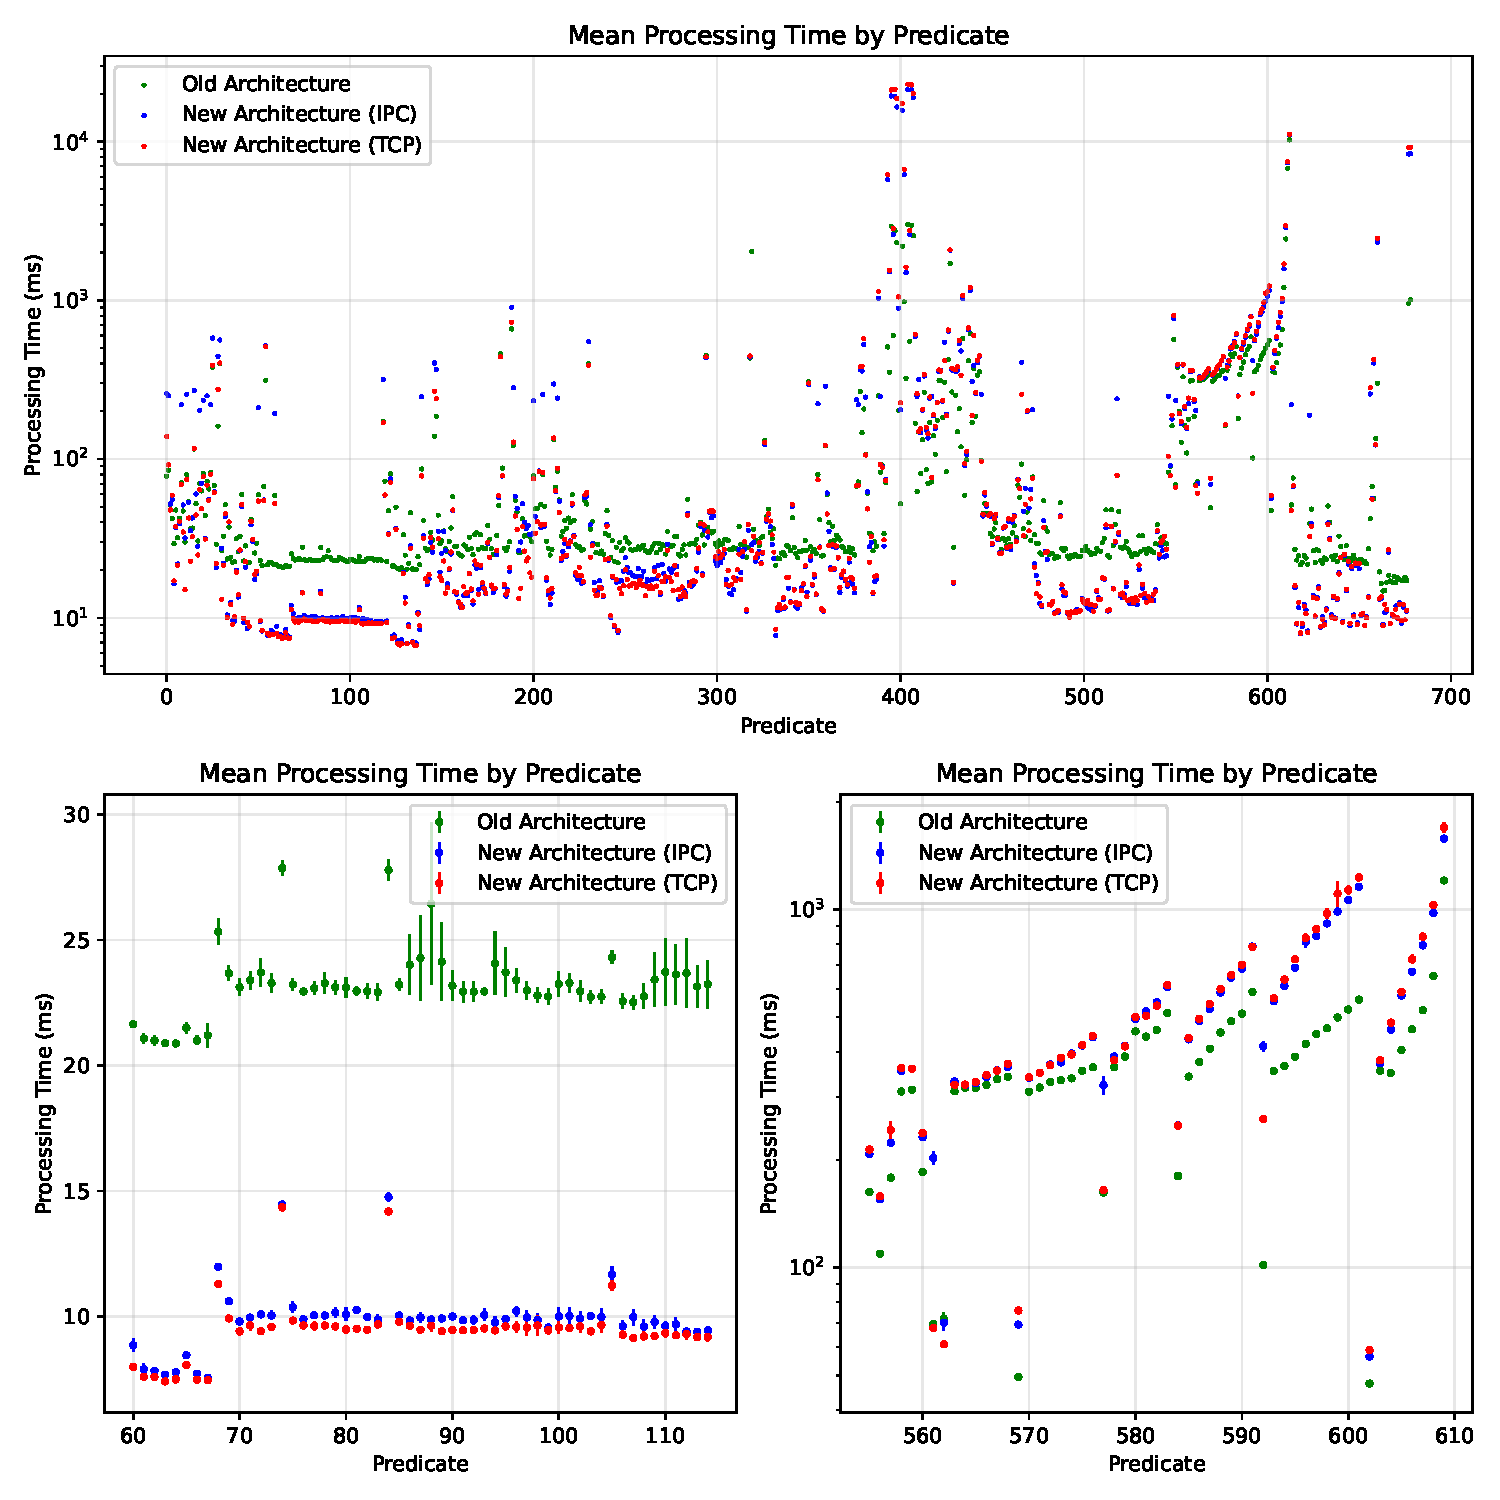
\includegraphics[scale=.55]{./PerformanceEvaluation/processingtime.pdf}
    \caption{Durchschnittliche Laufzeiten der Anfragen in den verschiedenen Architekturen.}
    \label{fig:performance-overview}
\end{figure}
% \FloatBarrier

Um sich zunächst einen Überblick über die Rohdaten zu verschaffen,
werden in \cref{fig:performance-overview} die durchschnittlichen Laufzeiten in den verschiedenen Konfigurationen dargestellt.
Der obere Subgraph zeigt die durchschnittlichen Laufzeiten aller Anfragen in sowohl der alten als auch der neuen Architektur,
wobei die neue Architektur in das IPC-Protokoll und TCP-Protokoll unterteilt ist.
Wider Erwarten zeigt sich, dass die durchschnittliche Laufzeit in der neuen Architektur bei vielen Prädikaten geringer ausfällt als in der alten Architektur.
Insgesamt sind von den 679 Prädikaten nur 172 Prädikate in der alten Architektur schneller gelöst worden.
265 Prädikate wurden in der IPC-Konfiguration und 242 Prädikate in der TCP-Konfiguration am schnellsten gelöst.

Die unteren beiden Subgraphen stellen interessante Bereiche der Rohdaten erneut dar und zeigen zusätzlich
die Standardfehler der Mittelwerte in Form der Fehlerbalken. Diese geben an, wie sehr die
Mittelwerte der Laufzeiten von den tatsächlichen Mittelwerten der Grundgesamtheit abweichen.
Kalkuliert wird dieser Standardfehler mittels der folgenden Formel:
\begin{equation}
    \sigma_{\overline{x}} = \frac{\sigma}{\sqrt{n}}
\end{equation}
Hierbei ist $\sigma_{\overline{x}}$ der Standardfehler des Mittelwertes, $\sigma$ die Standardabweichung der Grundgesamtheit und $n$ die Anzahl der Messungen.
Somit werden ausschließlich statistische Fehler betrachtet und systematische Fehler nicht berücksichtigt.

So zeigt der untere linke Subgraph die Rohdaten im Bereich der Prädikate 60 bis 115 erneut,
wobei klar zu erkennen ist, dass hier die neue Server-Architektur konstant schneller ist.
Dieser Trend ist über die gesamte Messung hin unterhalb einer gewissen Grenze zu beobachten.
Ebenfalls ersichtlich ist der nur minimal ausfallende Unterschied zwischen IPC und TCP.

Auf der anderen Seite zeigt der untere rechte Subgraph die Rohdaten im Bereich der Prädikate 555 bis 610.
Hier haben die Laufzeit Messungen einen vergleichsweise hohen Wert und es ist zu erkennen,
dass die alte Architektur in diesem Bereich schneller ist. 

Entsprechend wurde durch die Protokollkommunikation ein Performance-Overhead eingeführt, der sich in den Rohdaten dahingehend widerspiegelt,
dass Prädikate, welche bereits eine hohe Laufzeit aufgewiesen haben, nun in der neuen Architektur noch langsamer gelöst werden.
Neben diesem Overhead wurde jedoch eine signifikante Laufzeitverbesserung erworben, die bis zu einer gewissen Gesamtlaufzeitsgrenze den
Overhead nicht nur annulliert, sondern überkompensiert.
Insgesamt scheint die neu eingeführte Server-Architektur hinsichtlich der Laufzeitperformance um einen gewissen Faktor effizienter geworden zu sein.

Ebenfalls ist zu erkennen, dass der Unterschied zwischen IPC und TCP nur minimal ist und keine signifikanten Unterschiede aufweist.
Innerhalb der 679 Testprädikaten ist IPC in 365 ($53.76\%$) Fällen schneller als TCP und entsprechend TCP in 314 ($46.24\%$) Fällen schneller als IPC.
Da zur TCP-Kommunikation die Adresse  $tcp://127.0.0.1$ verwendet wurde, ist eine mögliche Erklärung hierfür, dass die Kommunikation über das Loopback-Interface
einen Großteil des Netzwerk-Stacks umgeht und vom Betriebssystem speziell optimiert wird.
In der weiteren Analyse wird daher nur das IPC-Protokoll betrachtet.

% \clearpage

Um den Overhead der neuen Architektur zu quantifizieren,
wird die Differenz der durchschnittlichen Laufzeiten der neuen ($\overline{t_\text{IPC}}$) und alten ($\overline{t_\text{Old}}$) Architektur berechnet
und gegen die Anzahl der ZeroMQ-Anfragen analysiert.
Der induzierte Overhead $t_\text{induced}$ wird also wie folgt definiert:

\begin{equation}
    t_\text{induced} = \overline{t_\text{IPC}} - \overline{t_\text{Old}}
\end{equation}

Der oberste Subgraph in \cref{fig:overhead} zeigt den induzierten Overhead der neuen Architektur in Abhängigkeit der Anzahl der ZeroMQ-Anfragen auf einer logarithmischen Skala.
Im groben Verlauf ist zu erkennen, dass der Overhead mit steigender Anzahl der Anfragen annähernd linear zunimmt.
Zusätzlich scheint jedoch eine ausgeprägte Systematik vorzuliegen, welche sich inhaltlich durch die horizontale Verzerrung der Daten ausprägt.
Einige wenige Datenpunkte weichen stark von jeglicher Systematik ab und sind als Ausreißer zu klassifizieren.

Im zweiten Subgraphen wird die lineare Abhängigkeit des Overheads von der Anzahl der Anfragen untersucht, indem der Zusammenhang linear gefittet\footnote{Der lineare Fit wurde mit dem von scipi.optimize bereitgestellten curve\_fit berechnet.} wird.
Dies geschieht unter Berücksichtigung des kombinierten Standardfehlers der Mittelwerte der alten und neuen IPC-Architektur.
Die Unsicherheitsberechnung wird berechnet mit der gaußschen Fehlerfortpflanzung

\begin{equation}
    \sigma_{\overline{comb}} = \sqrt{\sigma_{\overline{IPC}}^2 + \sigma_{\overline{Old}}^2} \hspace{0.3cm},
\end{equation}

welche ebenfalls in den Fehlerbalken dargestellt wird.
Das Ergebnis des linearen Fits zeigt eine Steigung von $0.03 ms$ pro Anfrage, was bedeutet, dass der Overhead pro Anfrage um $0.03 ms$ steigt.
Zusätzlich gibt es einen y-Achsenabschnitt von $-13.13 ms$, was bedeutet, dass der Overhead bei $0$ Anfragen $-13.13 ms$ beträgt.
Dieser Wert beschreibt die zuvor erfasste Laufzeitverbesserung der neuen Architektur.
Insgesamt ergibt sich die folgende lineare Funktion zur Beschreibung des Overheads:

\begin{equation}
    Overhead = 0.03ms \cdot Anfragenanzahl - 13.13ms
\end{equation}

Durch das Gleichsetzten der Overhead-Funktion mit $0$ ergibt sich eine Anzahl an Anfragen von etwa $438$, bis der Overhead nicht länger von der Laufzeitverbesserung kompensiert werden kann.

Eine separate Messreihe wurde durchgeführt, um die durchschnittliche Laufzeit einer einzelnen Anfrage an den Z3-Server zu ermitteln.
Hierbei wurde die durchschnittliche Laufzeit von $0.0054 ms$ bestimmt.
Da für jede Anfrage zwei Nachrichten (Anfrage und Antwort) über den Socket gesendet werden, ergibt sich eine Laufzeit von $0.0216 ms$ pro Anfrage
unter der Annahme, dass das Erhalten einer ZeroMQ-Nachricht die gleiche Laufzeit aufweist wie das Senden einer Nachricht.
Die Differenz von $0.0084 ms$ zur ermittelten Steigung des linearen Fits könnte beispielsweise auf die Größe der Nachrichten zurückzuführen, welche
in der kontrollierten Messreihe einer einzelnen Anfrage kleiner ausfällt als in den 52 Testszenarien.
Zudem sind Messwerte dieser Größenordnung zunehmend ungenau, weshalb sie annehmbar plausibel bezüglich der Steigung des linearen Fits sind.


\begin{figure}[!htp]
    \centering
    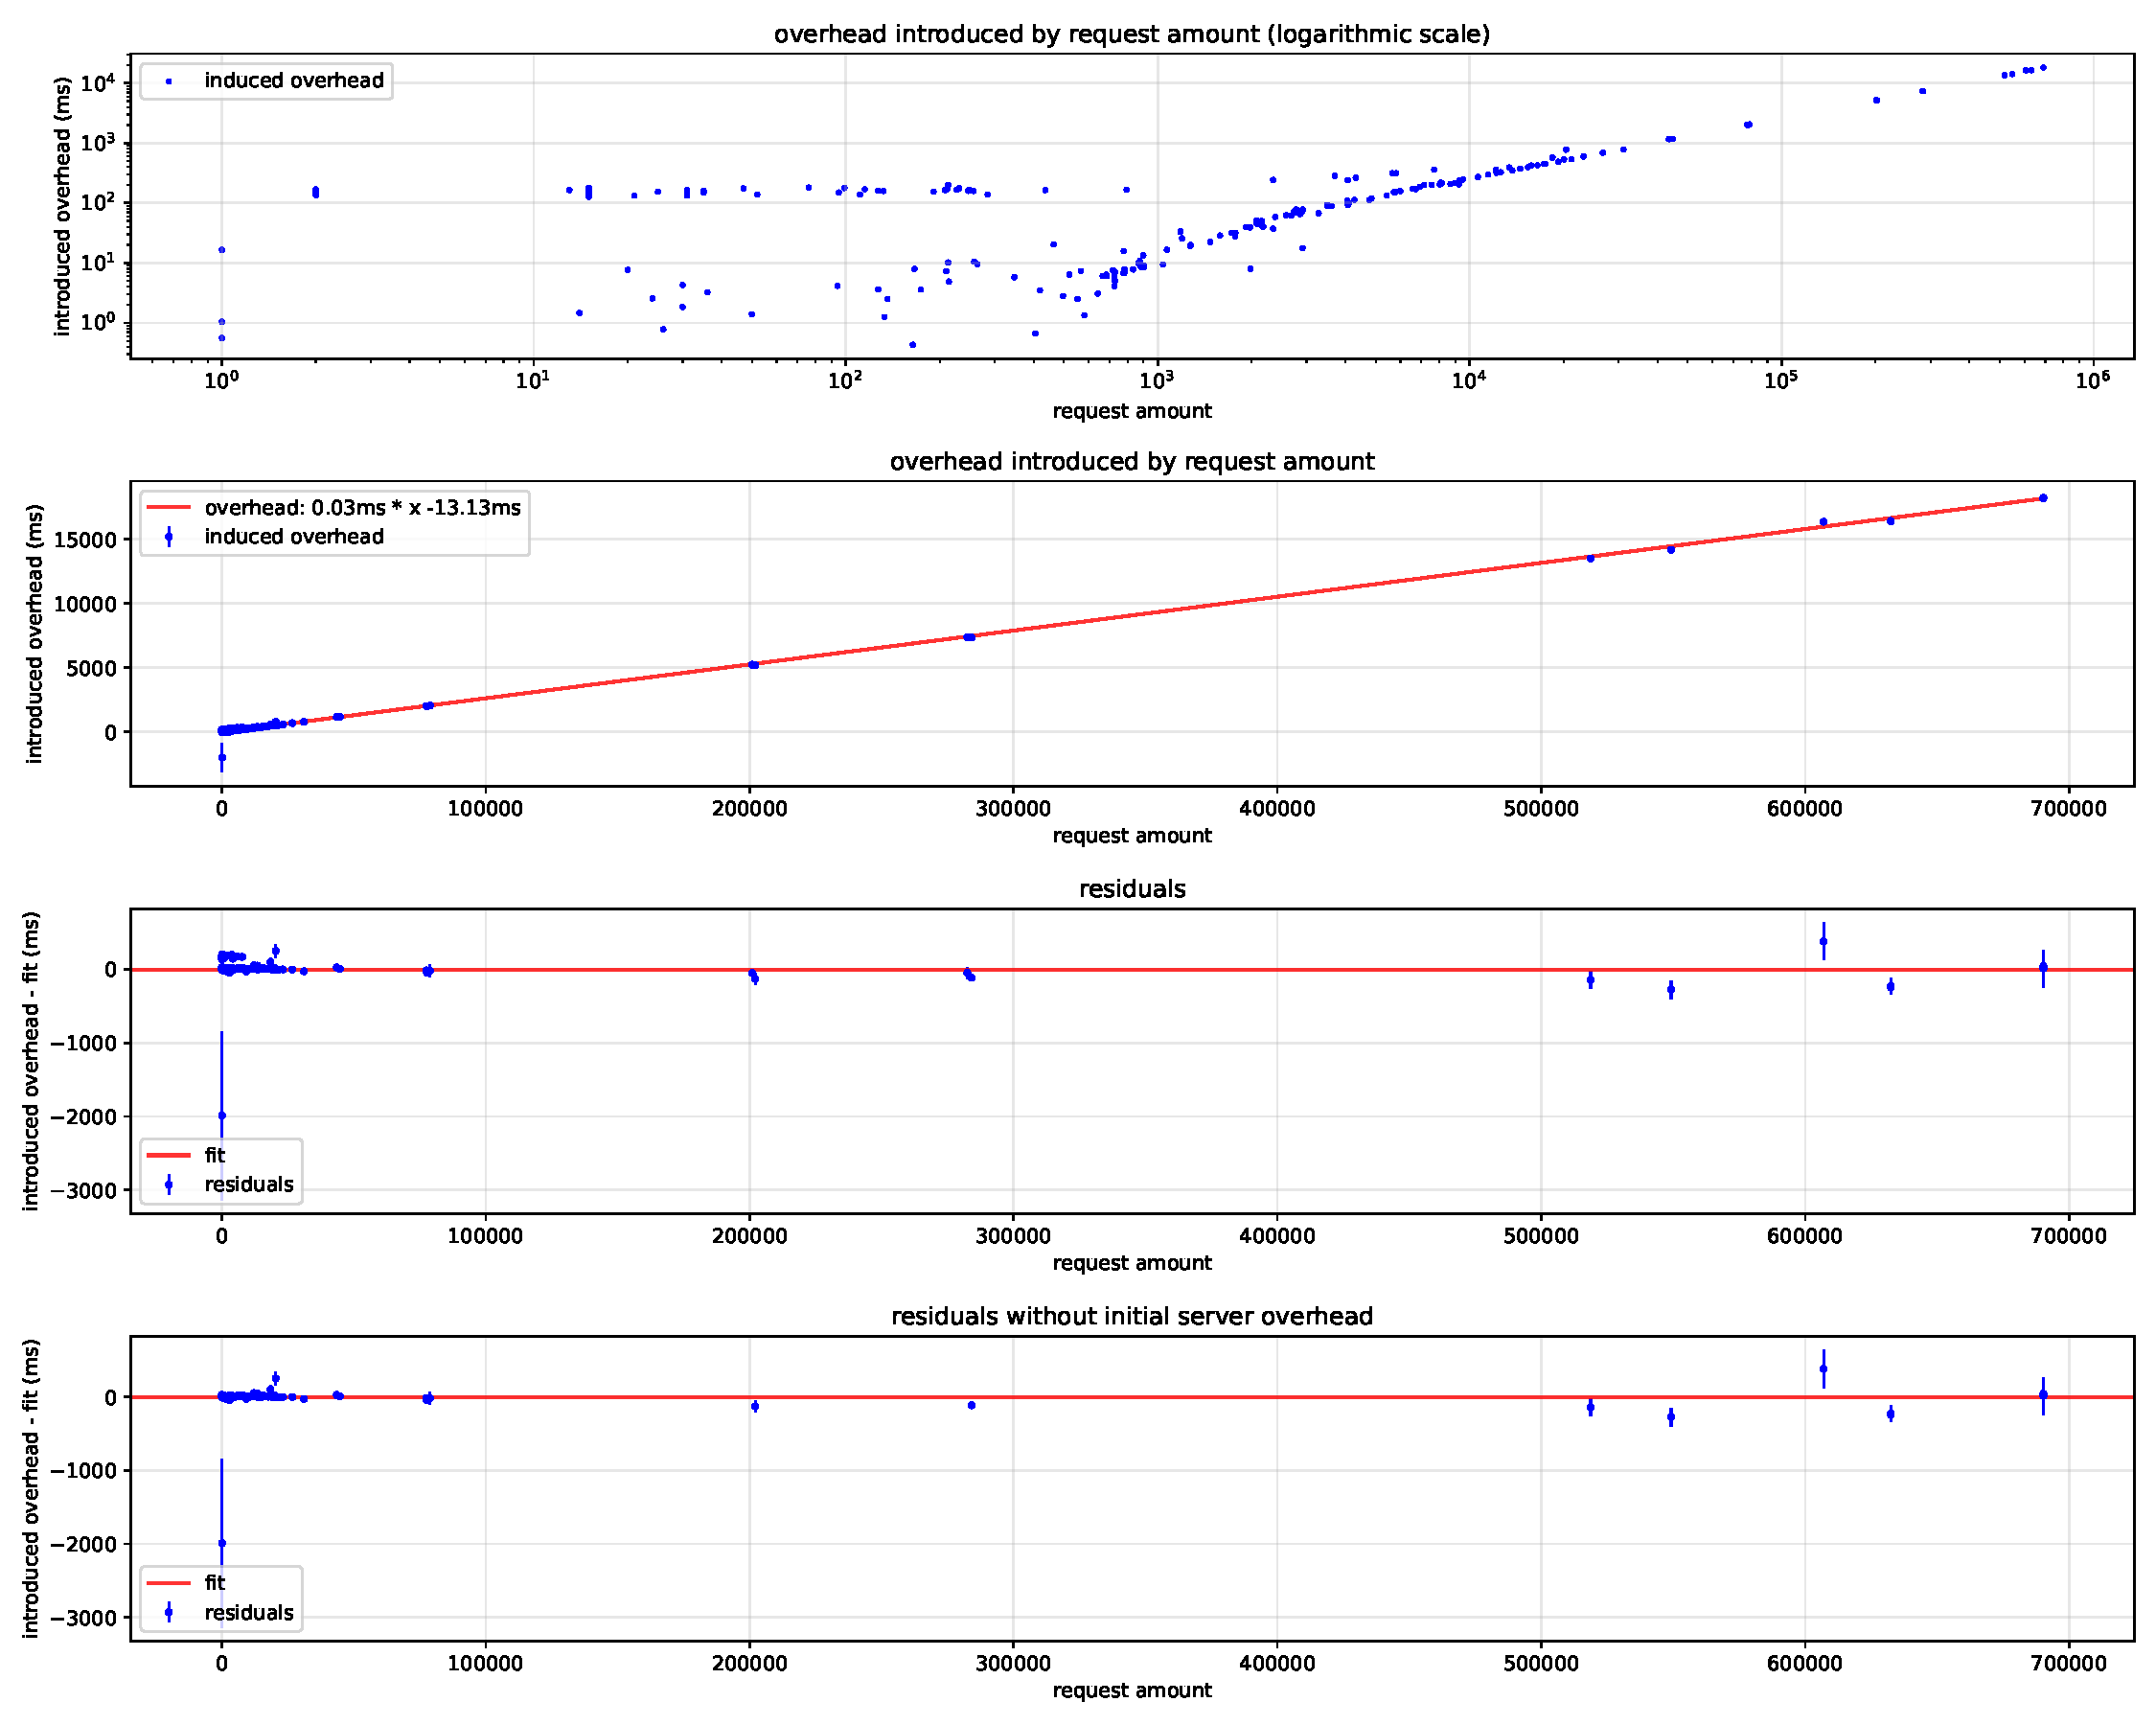
\includegraphics[scale=.55]{./PerformanceEvaluation/overhead.pdf}
    \caption{Induzierter Overhead der neuen Server-Architektur durch das Serialisieren auf den Socket.}
    \label{fig:overhead}
\end{figure}
% \FloatBarrier
% \clearpage

Der lineare Fit zeigt augenscheinlich eine gute Übereinstimmung mit den Daten, welche in dem dritten Subgraphen aus \cref{fig:overhead} verifiziert wird.
Hierbei wird die Differenz des induzierten Overheads und des linearen Fits gegen die Anzahl der Anfragen dargestellt.
Es ergibt sich ein Residuenplot.
In diesem Plot ist die Systematik des obersten Subgraphen erneut zu erkennen.
Sie bildet ein kleines Cluster oberhalb der $0$-Linie, bei sehr kleinen Anfragenzahlen.
Es stellt sich heraus, dass innerhalb dieses Datenclusters alle Datenpunkte die QueryID $1$ aufweisen.
Somit lässt sich die Abweichung durch das Initialisieren des Sockets, der Verbindung des Z3-Servers und dessen initialen Overheads zum Aufsetzten der Z3-Konfigurationen erklären.
Innerhalb einer TestID wird der Z3-Server nur einmalig initialisiert und folgende Prädikate desselben Tests nutzen denselben Z3-Server, indem sie die Konfiguration zurücksetzten und nicht grundlegend neu initialisieren.

Zur Überprüfung stellt der letzte Subgraph erneut den Residuenplot dar, jedoch ohne diejenigen Datenpunkte mit QueryID $1$.
Hierbei ist zu erkennen, dass die Systematik des vorherigen Graphen verschwindet und der lineare Fit eine gute Übereinstimmung mit den Daten aufweist.
Somit ist gezeigt, dass der Overhead der neuen Architektur durch das Serialisieren auf den Socket annähernd linear mit der Anzahl der Anfragen zunimmt
und keine weiteren relevanten Systematiken besitzt. Eine Voraussage des Overheads ist mithilfe des linearen Fits möglich.
Es ist zu beachten, dass die absoluten Werte des Overheads nur in der gegebenen Testumgebung gültig sind und nicht auf andere Umgebungen übertragen werden können.

Ein einzelner Datenpunkt scheint eine unwahrscheinlich hohe Laufzeitverbesserung von durchschnittlich $2$ Sekunden aufzuweisen, weist jedoch hohe Messunsicherheiten auf.
In \cref{tab:broken-datapoint} ist dieser Datenpunkt dargestellt.

\begin{table}[!htp]
    \centering
    \caption{Ausschnitt der gesammelten Messwerte eines Ausreißers.}
    \label{tab:broken-datapoint}
    \begin{tabular}{ cccccc }
        \toprule
        \textbf{TestID-QueryID} & \textbf{$Old_1(ms)$} & \textbf{$Old_2(ms)$} & \textbf{$Old_3(ms)$} & \textbf{$Old_4(ms)$} & \textbf{Req. Count} \\
        \midrule
        2122-90                 & 36                   & 4033                 & 3993                 & 43                   & 119                 \\
        \bottomrule
    \end{tabular}
\end{table}
% \FloatBarrier

Die verschiedenen Messwerte der alten Architektur in Millisekunden zeigen zwei starke Ausreißer bei der zweiten und dritten Messung.
Diese Varianz ist womöglich auf die in \cref{subsec:softlock} beschriebene Problematik zurückzuführen.
In jedem Fall ist dieser Datenpunkt als individueller Ausreißer zu betrachten und weist keine besondere statistische Relevanz auf.

Die ermittelte Performance-Verbesserung wird an dieser Stelle nicht weiter analysiert, da sie nicht Gegenstand dieser Arbeit ist.
Ein möglicher Grund für die Verbesserung könnte die Kompilierung sein, die durch die neue Architektur ermöglicht wird,
da der Z3-Solver als eigenständiger Prozess womöglich besser vom Compiler optimiert werden kann.
Als eigenständiger Prozess ist es ebenfalls möglich, dass der runtime linker die Z3-Bibliothek optimierter laden und ausführen kann.
Zusätzlich könnten die in \cref{subsec:optimizations} beschriebenen Optimierungen eine Rolle spielen.

\clearpage


\section{Zukünftige Arbeiten}


\subsection{Weitere Analyse und Optimierungen}

    analyse performance improvement

\subsection{Deinit Hook}

 deinit für dangling zocket und prozess (cleaner)

\subsection{Parallelisierung}

 threading in ProB (eigentlicher Sinn der Arbeit um zu parallelisieren)

\clearpage


\section{Konklusion}

stuff

% %%%%%%%%%%%%%%%%%%%%%%%%%%%%%%%%%%%%%%%%%%%%%%%%%%%%%%%%%%%%%%%%%%%%%%%%%%%%%%%%
% Diese Datei beinhaltet den eigentlichen Inhalt Ihrer Arbeit.
%
% Es bietet sich der Übersicht halber an, die einzelnen Abschnitte jeweils
% in eigene Dateien zu schreiben und mittels \input einzubinden.
% Eine mögliche Verzeichnisstruktur sähe entsprechend so aus:
%
%     thesis/
%     +- tex/
%     |  +- introduction.tex
%     |  +- motivation.tex
%     |  +- experiments.tex
%     |  |  ...
%     |  +- conclusion.tex
%     +- abstract.tex
%     +- contents.tex
%     +- thesis.tex
%%%%%%%%%%%%%%%%%%%%%%%%%%%%%%%%%%%%%%%%%%%%%%%%%%%%%%%%%%%%%%%%%%%%%%%%%%%%%%%%

\section{Einleitung}

Dies ist der Hauptteil Ihrer Arbeit.
Hier leiten Sie grob in das Thema ein, motivieren es und geben einen Ausblick
über das, was Sie in Ihrer Arbeit behandeln werden.

Der Inhalt der Vorlage ist mit Beispielen gefüllt, wie man \LaTeX{}
verwendet und traditionelle Stolpersteine vermeidet.
Lesen Sie die Vorlage gründlich.


\subsection{Makefile}

Im Wurzelverzeichnis finden Sie ein \texttt{Makefile}.
Über das Terminal können Sie die folgenden Befehle aufrufen,
wie in \cref{tab:make} beschrieben.


\begin{table}[h]
  \centering
  \caption{Übersicht der \texttt{Makefile}-Befehle.}%
  \label{tab:make}
  \begin{tabularx}{\textwidth}{lX}
    \toprule
    Befehl & Effekt \\
    \midrule
    \texttt{make} & Kompiliert das PDF und löscht aux-Files. \\
    \texttt{make clean} & Löscht das PDF und dazugehörige aux-Files. \\
    \texttt{make bibtool} & Sortiert \texttt{references.bib}
    und formatiert die Einträge einheitlich. \\
    \texttt{make watch} & Rekompiliert das PDF bei Änderungen und
    hält die Anzeige in Ihrem PDF-Betrachter aktuell. \\
    \bottomrule
  \end{tabularx}
\end{table}


\section{Referenzen und Zitationen}

In der Datei \texttt{references.bib} finden Sie bereits einige Quellen,
die Sie wahrscheinlich zitieren mögen,
wie z.B. die B Methode~\cite{abrial1996b,abrial2010modeling}
oder \textsc{ProB}~\cite{leuschel2003prob,leuschel2008prob}.
Beachten Sie den Artikel ``Common Errors in Bibliographies'' von John Owens.%
\footnote{\url{https://www.ece.ucdavis.edu/~jowens/biberrors.html}}
Zusätzliche, ausführlichere Informationen finden Sie auch in \cref{app:sec:bib}.


\subsection{Referenzen platzieren}

Sie platzieren Referenzen mit \texttt{\textbackslash{}cite{}}.
Diese sollten jeweils hinter dem Namen der zitierten Technik stehen,
oder hinter der zu belegenden Aussage.
Im Falle, dass sich ein gesamter Absatz auf eine einzelne Quelle bezieht,
genügt es die Referenz im ersten Satz anzugeben, solange vom Kontext klar ist,
dass der restliche Absatz sich ebenfalls auf die Quelle bezieht.
Referenzen sind nicht erst am Ende eines gesamten Absatzes zu platzieren.
Ebenso sind sie Teil des Satzes und stehen vor dem abschließenden Punkt.

\begin{itemize}
  \item Gut: \enquote{\textsc{ProB}~\cite{leuschel2003prob} is an
    animator, model checker, and constraint solver for the B method~\cite{abrial1996b}.
    The B method allows to specify, design, and code
    software systems as well as to perform formal proof of their properties.}
  \item Nicht gut: \enquote{\textsc{ProB} is an
    animator, model checker, and constraint solver for the B method~\cite{leuschel2003prob,abrial1996b}.
    The B method allows to specify, design, and code
    software systems as well as to perform formal proof of their properties.}
  \item Nicht gut: \enquote{\textsc{ProB} is an
    animator, model checker, and constraint solver for the B method
    The B method allows to specify, design, and code
    software systems as well as to perform formal proof of their properties.~\cite{leuschel2003prob,abrial1996b}}
\end{itemize}


\subsection{Über Literatur sprechen}

Obwohl die Referenzen innerhalb des Satzes stehen, sind sie keine Wörter.
Sie ersetzen somit nicht die explizite Nennung einer Quelle.
Sollte über ein bestimmtes Papier gesprochen werden, so ist dieses via
Autorennamen zu betiteln. Hierbei gilt:
\begin{itemize}
  \item Es sind nur die Nachnamen zu verwenden,
  \item hinter den Autorennamen ist die Referenz zu setzen,
    falls der Bezug unklar ist,
  \item ab drei oder mehr Autoren wird nur der Erstautor geführt, gefolgt von
    \enquote{et al.}.
\end{itemize}

So schreiben wir
\enquote{SICStus Prolog~\cite{carlsson1988sicstus} wurde von Carlson et al.\
  entwickelt}
oder
\enquote{Leuschel \& Butler~\cite{leuschel2003prob} haben einen Model Checker für die
  B-Methode~\cite{abrial1996b} entwickelt}.
Falsch hingegen ist es, eine Referenz als eigenständiges Wort zu nutzen, wie in
folgendem Negativbeispiel:
\enquote{In \cite{leuschel2003prob} wurde ein Model Checker für die B-Methode entwickelt}.



\section{Bilder und Tabellen}

Bilder und Tabellen sind per se wie von \LaTeX{} bekannt zu setzen.
Wichtig ist, dass sie ausnahmslos im Fließtext referenziert wurden.
Eine nichtreferenzierte Tabelle oder Abbildung kann ebenso ausgelassen werden.
Solche Querverweise werden in \cref{sec:references} besprochen.


\subsection{Bilder}%
\label{sec:figures}

\Cref{fig:initial-draft} ist eine exemplarische Abbildung, auf die an dieser
Stelle im Text verwiesen wird.
Stilistisch ist es meist empfehlenswert innerhalb der
\texttt{figure}-Umgebung ein \texttt{\textbackslash{}centering} zu setzen,
sodass der Inhalt zentriert wird.
In \cref{fig:hhu-logo} wird ein Beispiel der
\texttt{\textbackslash{}subfigure}-Umgebung aus dem
\texttt{\textbackslash{}subcaption}-Paket demonstriert.
Beide Teilabbildungen, \cref{fig:hhu-rgb,fig:hhu-bw},
sind individuell referenzierbar.

\begin{figure}[h]
  \centering
  
\includegraphics[width=4cm]{fig/the.png}
  \caption{Initial thesis draft.}%
  \label{fig:initial-draft}
\end{figure}

\begin{figure}[h]
  \begin{subfigure}{.5\textwidth}
    \centering
    
\includegraphics[width=4cm]{fig/hhu-logo-rgb.pdf}
    \subcaption{in Farbe}%
    \label{fig:hhu-rgb}
  \end{subfigure}% <- Kommentarzeichen am Ende der Zeile ist wichtig!
  \begin{subfigure}{.5\textwidth}
    \centering
    
\includegraphics[width=4cm]{fig/hhu-logo-black.pdf}
    \subcaption{Schwarzweiß}%
    \label{fig:hhu-bw}
  \end{subfigure}% <- Kommentarzeichen am Ende der Zeile ist wichtig!
  \caption{Das neue HHU-Logo.}%
  \label{fig:hhu-logo}
\end{figure}


\subsection{Tabellen}%
\label{sec:tables}

Während bei Abbildungen die \texttt{\textbackslash{}caption}
in aller Regel unter dem Bild steht,
wird sie bei Tabellen typischer Weise darüber platziert, wie bei
\cref{table:truths} zu sehen.

\begin{table}[ht]
  \begin{center}
    \caption{Table of truths.}%
    \label{table:truths}
    \begin{tabular}{lr}
      \toprule
      Fakt                                & Wahrheitsgehalt \\
      \midrule
      booktabs-Tabellen sind hübscher     & 90 \%           \\
      Han Solo schoss zuerst              & 100 \%          \\
      Game of Thrones fand ein gutes Ende & 0 \%            \\
      \bottomrule
    \end{tabular}
  \end{center}
\end{table}

Es ist zu empfehlen, das Paket \texttt{booktabs} zur Formatierung der Tabellen
zu nutzen.
Dieses empfiehlt die Verwendung der Befehle
\texttt{\textbackslash{}toprule},
\texttt{\textbackslash{}midrule} und
\texttt{\textbackslash{}bottomrule},
und rät davon ab, vertikale Linien zu nutzen.
Vergleichen Sie \cref{tab:booktabs-yes,tab:booktabs-yesnt}.

\begin{table}
  \centering
  \caption{Vergleich von \LaTeX{}-Tabellen mit und ohne booktabs.}
  \begin{subtable}{.5\textwidth}
    \centering
    \subcaption{mit booktabs}%
    \label{tab:booktabs-yes}
    \begin{tabular}{lrr}
      \toprule
      Backend & Accuracy & F\textsubscript{1}-Score \\
      \midrule
      CLP(FD) & 0.947 & 0.966 \\
      Z3      & 0.919 & 0.797 \\
      \bottomrule
    \end{tabular}
  \end{subtable}%
  \begin{subtable}{.5\textwidth}
    \centering
    \subcaption{ohne booktabs}%
    \label{tab:booktabs-yesnt}
    \begin{tabular}{|l|r|r|}
      \hline
      Backend & Accuracy & F\textsubscript{1}-Score \\ \hline
      CLP(FD) & 0.947 & 0.966 \\ \hline
      Z3      & 0.919 & 0.797 \\ \hline
    \end{tabular}
  \end{subtable}%
\end{table}



\subsection{Plots}%
\label{sec:plot}

Sie können mithilfe von \texttt{tikz} und \texttt{pgfplots}
Graphen oder Bar Charts erstellen,
wie in \cref{fig:the-plot,fig:long-caption} der gezeigt ist.
Beachten Sie, dass die Vorlage die Cycle Lists
\texttt{hhubwcycle} (schwarzweiß) und \texttt{hhucolorcycle} bereit stellt,
welche die offiziellen HHU-Farben zur Darstellung der verschiedenen Graphen
verwendet.
Diese können in jeglichem \texttt{tikzplot} mittels der Option
\texttt{cycle list name=} gesetzt werden und stehen, je nach Druckeinstellung
innerhalb der PDF via \texttt{\textbackslash{}blackwhiteprint}
entweder automatisch auf \texttt{hhucolorcycle} oder \texttt{hhubwcycle}.

\begin{figure}[ht]
  \centering
  \begin{subfigure}{.5\textwidth}
    \centering
    \begin{tikzpicture}
      \begin{axis}[
        width=\textwidth,
        cycle list name=hhucolorcycle
      ]
        \foreach \y in {0,0.1,...,1} % Wiederholt \addplot mit jeweils anderem \y
          \addplot coordinates {
              ( 1, 3.0 -\y)
              ( 2, 3.25-\y)
              ( 3, 3.5 -\y)
              ( 4, 3.75-\y)
              ( 5, 4.0 -\y)
            };
      \end{axis}
    \end{tikzpicture}
    \subcaption{in den HHU-Farben}
  \end{subfigure}%
  \begin{subfigure}{.5\textwidth}
    \centering
    \begin{tikzpicture}
      \begin{axis}[
        width=\textwidth,
        cycle list name=hhubwcycle % <- Änderung auf schwarzweiß.
      ]
        \foreach \y in {0,0.1,...,1} % Wiederholt \addplot mit jeweils anderem \y
          \addplot coordinates {
              ( 1, 3.0 -\y)
              ( 2, 3.25-\y)
              ( 3, 3.5 -\y)
              ( 4, 3.75-\y)
              ( 5, 4.0 -\y)
            };
      \end{axis}
    \end{tikzpicture}
    \subcaption{in schwarzweiß}
  \end{subfigure}%
  \caption{A beautiful plot.}%
  \label{fig:the-plot}
\end{figure}

\begin{figure}[ht]
  \centering
  \begin{tikzpicture}
    \begin{axis}
      [
        ybar,
        xtick=data,
        enlarge x limits=1,
        symbolic x coords={A, B},
        ymin=0, ymax=100,
        ylabel={$\%$ percentage of bar height},
      ]
      \addplot coordinates {(A,90) (B, 90)};
      \addplot coordinates {(A,75) (B, 75)};
      \addplot coordinates {(A,60) (B, 60)};
      \addplot coordinates {(A,45) (B, 45)};
      \addplot coordinates {(A,30) (B, 30)};
      \legend{blue, orange, green, red, cyan}
    \end{axis}
  \end{tikzpicture}
  \caption[Bar plot with short version of caption for List of Figures]{%
    A really long caption title. This demonstrates how to describe stuff seen
    in the figure, like here, where we see a bar plot showing my favourite
    pies. Nah, actually it shows something completely different.
  }\label{fig:long-caption}
\end{figure}



\section{Querverweise}\label{sec:references}

Für Querverweise, wie zu
\cref{fig:initial-draft,fig:hhu-logo,fig:the-plot,fig:long-caption},
\cref{lst:hello-c,lst:hello-prolog}
oder \cref{alg:minimax}
stehen zwei Möglichkeiten zur Verfügung:
die \LaTeX{}-Standardvariante via \texttt{\textbackslash{}ref},
oder (eleganter) das \texttt{cleveref}-Paket.

Cleveref ermittelt automatisch, welche Art von Element referenziert wird
und fügt den entsprechenden Titel hinzu. Entsprechend sind die in
\cref{tab:cleveref} aufgeführten Beispiele äquivalent.

\begin{table}[ht]
  \centering
  \caption{Vergleich \texttt{\textbackslash{}ref} und \texttt{\textbackslash{}cref}.}%
  \label{tab:cleveref}
  \begin{tabularx}{\textwidth}{XX}
    \toprule
    \LaTeX{} & Darstellung \\
    \midrule
    \lstinline[language=tex]|Abbildung \\ref\{fig:logo\} zeigt das Logo.| &
      Abbildung \ref{fig:hhu-logo} zeigt das Logo. \\
    \lstinline[language=tex]|\\cref\{fig:logo\} zeigt das Logo.| &
      \cref{fig:hhu-logo} zeigt das Logo. \\
    \addlinespace
    \lstinline[language=tex]|Abbildungen \\ref\{fig:plot1\} und|
      \lstinline[language=tex]|\\ref\{plot2\} sind Graphen.| &
    Abbildungen \ref{fig:the-plot} und \ref{fig:long-caption} sind Graphen.\\
    \lstinline[language=tex]|\\Cref\{fig:plot1,plot2\} sind Graphen.| &
    \Cref{fig:the-plot,fig:long-caption} sind Graphen.\\
    \bottomrule
  \end{tabularx}
\end{table}



\section{Formeln}

\Cref{eq:example1} gibt eine referenzierbare Formel an,
während \cref{eq:example2} eine Formel darstellt, die länger ist, als die
Zeile zulässt.

\begin{equation}
  \label{eq:example1}
  2 = 1 + 1
\end{equation}

\begin{multline}
  \label{eq:example2}
  30 = 1 + 1 + 1 + 1 + 1 + 1 + 1 + 1 + 1 + 1 + 1 + 1 + 1 + 1 + 1 + 1 + 1 + 1 \\
      + 1 + 1 + 1 + 1 + 1 + 1 + 1 + 1 + 1 + 1 + 1 + 1
\end{multline}

In der zweizeiligen Gleichung
\begin{equation}
  \label{eq:mlp-stacking}
  \begin{split}
    \hat{y} & = f_2(f_1(x; W); V) \\
            & = f(x; W, V)
  \end{split}
\end{equation}
wurden die Gleichheitszeichen in beiden Zeilen direkt untereinander ausgerichtet
(mittels \texttt{\&} im Quelltext und der \texttt{split}-Umgebung).
Teilen wir \cref{eq:mlp-stacking}, welche den Forward Pass eines Neuronalen
Netzes darstellt,
in mehrere Schritte auf, so erhalten wir (mittels \texttt{align}-Umgebung)
\begin{align}
  a       & = W^\mathsf{T} x \label{eq:fp-act} \\
  h       & = g_1(a) \label{eq:fp-hidden} \\
  o       & = V^\mathsf{T} h \label{eq:fp-out} \\
  \hat{y} & = g_2(o) \label{eq:fp-pred}
  \,\text{,}
\end{align}
wobei \cref{eq:fp-act,eq:fp-hidden,eq:fp-out,eq:fp-pred} jeweils eine eigene
Referenznummer erhalten.


\section{Algorithmen}

Für Algorithmen kann das bereits inkludierte Paket \texttt{algorithmicx}
genutzt werden.
In \cref{alg:minimax} wird exemplarisch eine Implementierung des
Minimax-Algorithmus aufgeführt.
Beachten Sie, dass \cref{line:commented} kommentiert und referenzierbar ist.

\begin{algorithm}
  \caption{Determining the next action by Minimax}%
  \label{alg:minimax}
  \begin{algorithmic}[1]
    \Function{Minimax}{Game State Tree: $G^n$}
      \State bestValue \(\gets -\infty\)
      \State \(\mathit{bestAction} \gets \) NIL
      \ForAll{\(G^n_a \in S(G^n)\)}
        \State \(\mathit{value} = \) \Call{MinimaxValue}{\(G^n_a\), true}
        \If{\(\mathit{value} > \mathit{bestValue}\)}
          \Comment{Aktualisiere besten Wert}\label{line:commented}
          \State \(\mathit{bestValue} \gets \mathit{value}\)
          \State \(\mathit{bestAction} \gets a\)
        \EndIf
      \EndFor
      \State \Return \(\mathit{bestAction}\)
    \EndFunction
    \Statex
    \Function{MinimaxValue}{Game State Tree: $G^n$, Boolean: $\mathit{ourTurn}$}
      \If{\(D(G^n)=0\)}
        \State \Return \Call{Heuristic}{root(\(G^n\))}
      \ElsIf{\(\mathit{ourTurn}\)}
        \State \(\mathit{maxValue} \gets -\infty \)
        \ForAll{\(S \in S(G^n)\)}
          \State \(\mathit{newValue} \gets \) \Call{MinimaxValue}{\(S\), false}
          \State \(\mathit{maxValue} \gets
            \max(\mathit{newValue}, \mathit{maxValue})\)
        \EndFor
        \State \Return \(maxValue\)
      \Else
        \State \(minValue \gets +\infty \)
        \ForAll{\(S \in S(G^n)\)}
          \State \(\mathit{newValue} \gets \) \Call{MinimaxValue}{\(S\), true}
          \State \(\mathit{minValue} \gets
            \min(\mathit{newValue}, \mathit{minValue})\)
        \EndFor
        \State \Return \(minValue\)
      \EndIf
    \EndFunction
  \end{algorithmic}
\end{algorithm}


\section{Source Code Listings}

\Cref{lst:hello-c,lst:hello-python} zeigen ein `Hello World'-Programm,
je in C und Python.
\Cref{lst:hello-prolog} zeigt ein Prolog-Prädikat, welches eine Liste in zwei
Teile teilen kann.

\begin{lstlisting}[
  float, caption={Hello World in C.}, label={lst:hello-c}, language=C
]
#include <stdio.h>

int main(int argc, char[] *args){
  printf("Hello World!\n");
  // And done!
}
\end{lstlisting}

\begin{lstlisting}[
  float, caption={Totally minimal Hello World in Python.},
  label={lst:hello-python}, language=Python
]
def hello_world():
  print("Hello World"!)

if __name__ == "__main__":
  hello_world()
\end{lstlisting}

\begin{lstlisting}[
  float, caption={Prolog implementation of \texttt{split/4}},
  label={lst:hello-prolog}, language=Prolog
]
% Split list into two parts (length of first list given).
%
% ?- split([a,b,c,d,e,f,g,h,i,k], 3, L1, L2).
% L1 = [a,b,c]
% L2 = [d,e,f,g,h,i,k]
%
split(L, N, L1, L2) :-
  length(L1, N),
  append(L1, L2, L).
\end{lstlisting}


\section{Todonotes}

Es bietet sich an, während der Verschriftlichung Gebrauch von dem
\texttt{todonotes}-Package zu machen.\todo[]{Lernen, wie man mit todonotes umgeht.}

Abgesehen davon, dass es erlaubt die PDF mit offenen Todos zu annotieren,
sind sie ein guter Weg um potentziellen Korrekturlesern zu kommunizieren,
welche Teile ohnehin noch nicht ausgearbeitet sind.
Des Weiteren lässt sich mit
\texttt{\textbackslash{}listoftodos} eine Übersicht der noch offenen Todos
im Dokument anzeigen

\listoftodos

\todo[inline]{Lerne was man machen kann, wenn man einzeln stehende Todos braucht.}
\todo[inline]{Lerne ebenfalls, \texttt{\textbackslash missingfigure} zu nutzen.}
\todo[inline]{Verschaffung eines Überblicks der in der Vorlage inkludierten Pakete.}


\subsection{Missingfigure}

Mittels \texttt{\textbackslash{}missingfigure} lassen sich bereits Abbildungen
im PDF darstellen, die noch erstellt werden müssen. Dies ermöglicht bereits einen
ersten Eindruck, wie das Layout um die Abbildung herum aussehen wird,
wie \cref{fig:missing} exemplarisch zeigt.

\begin{figure}
  \centering
  \missingfigure{Plot is still to be done, but the results from the HPC are not
    yet available.}
  \caption{Finale Laufzeiten meiner unfassbar guten Auswertung.}%
  \label{fig:missing}
\end{figure}


\section{Häufige Fehler}

Der wohl häufigste Fehler, den neue \LaTeX-Nutzer machen, ist eine falsche
Verwendung von Anführungszeichen.
Um dem Vorzubeugen sowie konsistente Anführungszeichen zu nutzen,
empfehlen wir den Einsatz von \texttt{\textbackslash{}enquote}
aus dem bereits inkludierten \texttt{csquotes}-Pakt.
% Dieses erlaubt ebenfalls eine gezielte und automatische Unterscheidung
% zwischen den \foreignquote{english}{englischen} und
% \foreignquote{german}{deutschen} Anführungszeichen.
Wird hingegen, wie in der Programmierung üblich, \textquotedbl verwendet,
versucht \LaTeX{} daraus einen Umlaut zu erzeugen.
So wird beispielsweise \texttt{\textquotedbl{}a} zu ä.

\Cref{tab:quotes} gibt eine Übersicht über verschiedene Möglichkeiten
Anführungszeichen zu setzen und demonstriert die falsche Verwendung von
\textquotedbl.

\begin{table}[ht]
  \centering
  \caption{Demonstration von csquotes.}%
  \label{tab:quotes}
  \begin{tabularx}{\textwidth}{XX}
    \toprule
    \LaTeX{} & Darstellung \\
    \midrule
    \texttt{Ein \textquotedbl{}Wort\textquotedbl{} in \textquotedbl{}Anführungszeichen\textquotedbl{}} &
      Ein "Wort" in "Anführungszeichen" \\ \addlinespace
    \texttt{Ein \textbackslash{}glqq Wort
        in \textbackslash{}glq Anführungszeichen\textbackslash{}grq\textbackslash{}grqq}&
      Ein \glqq Wort in \glq Anführungszeichen\grq\grqq \\ \addlinespace
    \texttt{Ein \textbackslash{}enquote\{Wort
        in \textbackslash{}enquote\{Anführungszeichen\}}\} &
      Ein \enquote{Wort in \enquote{Anführungszeichen}} \\
    \bottomrule
  \end{tabularx}
\end{table}

\section{Conclusion}

Am Ende der Arbeit werden noch einmal die erreichten Ergebnisse
zusammengefasst und diskutiert.


%% Dieser Part kann auskommentiert werden, sollte kein Anhang nötig sein.
%% Der \appendix-Befehl leitet hierbei den Anhang ein.
%  \appendix
%  \section{Zusätzliche Informationen}

Hier können Sie Ihren Anhang definieren.

Achten Sie darauf, dass der Anhang in Ihrer \texttt{thesis.tex}
initial auskommentiert ist.
Der entsprechende Part befindet sich nahe dem Ende der Datei.
Entfernen Sie bei Bedarf die Kommentierung um den Anhang nutzen zu können.


\section{Nutzung}

Der Anhang wird wie die Abschnitte des Hauptteils der Arbeit gestaltet,
also mit \texttt{\textbackslash section} Befehlen.

  \subsection{Unterabschnitte}
  Die Verwendung von Unterabschnitten im Anhang
  mittels \texttt{\textbackslash subsection}
  funktioniert ebenfalls!

\section{Bibliographie}%
\label{app:sec:bib}

Während ihrer Literatur-Recherche werden Sie vermutlich hauptsächlich auf vier Arten
an Quellen stoßen, die Sie in der \verb|.bib|-Datei unterbringen:
Konferenz-Artikel, Sammlungen an Kapiteln von mehreren Autoren, Journal-Artikel und Monographien.
Manche Bibtex-Einträge (etwa von Google Scholar) enthalten nicht alle Informationen
bzw. nicht im selben Format.

\textbf{Wichtig: Eine saubere Bibliographie besteht aus vollständigen und einheitlichen Einträgen!}

Im Folgenden wird beschrieben, was Sie hier für eine möglichst saubere Literaturliste beachten sollten.

\subsection{Konferenzartikel}

In der Informatik wird die meiste Forschung auf Konferenzen vorgestellt.
Hier reichen Autoren ihre Arbeiten ein, andere Forscher begutachten diese
und anhand dessen werden die besten Arbeiten für Konferenzvorträge ausgewählt.
In der Regel gibt es dazu Tagungsbände, die sogenannten \emph{Proceedings},
in denen die vorgestellten Forschungsartikel gesammelt werden.

\begin{figure}
    \centering
    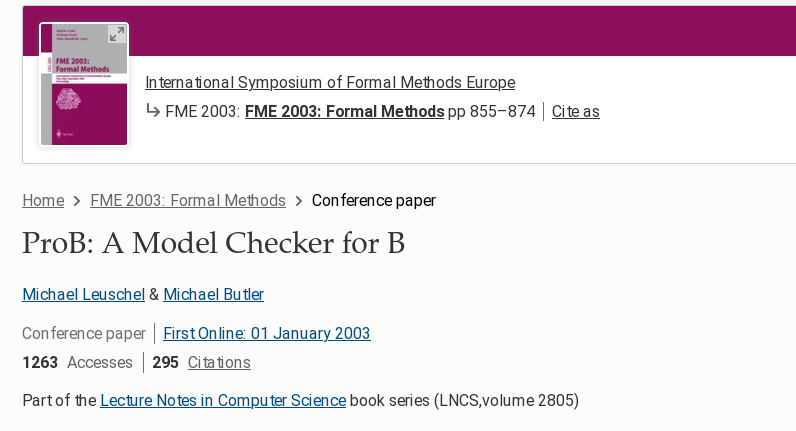
\includegraphics[scale=.5]{fig/prob-springer.png}
    \caption[Screenshot von \url{https://link.springer.com}]{
      Screenshot von \url{https://link.springer.com/chapter/10.1007/978-3-540-45236-2_46}}%
    \label{fig:prob-springer}
\end{figure}

Ein Beispiel ist der Artikel von Leuschel und Butler zu \textsc{ProB}~\cite{leuschel2003prob}.
In \cref{fig:prob-springer} sind die wichtigen Informationen für den Bibtex-Eintrag zu finden,
die Sie auf jeden Fall angeben sollten.
Ein Beispiel für einen passenden Bibtex-Eintrag lautet wie folgt (hier wird der \verb|InProceedings|-Typ verwendet):

\begin{verbatim}
@InProceedings(leuschel2003prob,
  Author	= {Leuschel, Michael and Butler, Michael},
  Title		= {{ProB}: A Model Checker for {B}},
  Year		= 2003,
  Month		= sep,
  Booktitle	= {{FME} 2003: Formal Methods},
  Series	= {LNCS},
  Volume	= 2805,
  Pages		= {855--874},
  Publisher	= {Springer},
  Address	= {Berlin, Heidelberg}
)
\end{verbatim}

\paragraph{Title, Author, Pages.} Diese Einträge sollten selbsterklärend sein.
\paragraph{Booktitle.} Hier gibt es mehrere valide Möglichkeiten.
Auf dem Buch selbst steht \enquote{FME 2003: Formal Methods}.
Akzeptabel wären auch \enquote{Proceedings FME 2003},
\enquote{Proceedings Formal Methods Europe (2003)},
\enquote{International Symposium of Formal Methods Europe. Pisa Italy, September 8-14, 2003, Proceedings}
oder Mischformen.
Wichtig ist, dass erkenntlich ist, zu welcher Konferenz aus welchem Jahr der Tagungsband stammt.
\paragraph{Year.} Leider erscheinen die Proceedings nicht unbedingt im selben Jahr wie die Konferenz selbst.
Daher ist auch das Jahr der Veröffentlichung anzugeben.
\paragraph{Series und Volume}. Proceedings vom Springer-Verlag erscheinen in der Regel in einer Reihe.
Üblich sind die LNCS (Lecture Notes in Computer Science). Darin erhalten sie auch eine Nummer, um sie eindeutig zu identifizieren.
Es gibt aber auch andere Reihen (z.B. LNAI oder CCIS); manchmal werden Tagungsbände auch mehreren Reihen zugeordnet.
Andere Herausgeber haben keine solche Reihe --- dann fallen diese Einträge weg.
\paragraph{Publisher.} Der Herausgeber der Proceedings.
Die meisten Tagungsbände werden vom Springer-Verlag oder der ACM veröffentlicht.
Hier gibt es auch mehrere valide Angaben (z.B. \enquote{Springer} bzw. \enquote{Springer-Verlag} oder \enquote{ACM} bzw. \enquote{Association for Computing Machinery}).
Diese sollten in Ihrer Bibliographie einheitlich sein.



\subsection{Sammelbände}

Es gibt einige Sammlungen an Artikeln, die als thematisches Buch veröffentlicht werden,
allerdings nicht aus einer Konferenz entstehen.
Ein Beispiel ist die Festschrift zu Egon Börgers 75.\ Geburtstag.
Darin findet man unter anderem den folgenden Artikel:

\begin{verbatim}
@InCollection(Leuschel2021,
  Author    = {Leuschel, Michael},
  Title     = {Spot the Difference: A Detailed Comparison Between {B}
                and Event-{B}},
  Booktitle = {Logic, Computation and Rigorous Methods},
  Publisher = {Springer},
  Year      = 2021,
  Volume    = 12750,
  Series    = {Lecture Notes in Computer Science},
  Pages     = {147--172}
)
\end{verbatim}

Insgesamt ist dies sehr ähnlich zum Konferenzartikel; deshalb wird her nicht näher auf die einzelnen Schlüssel eingegangen.
Auch dieses Buch wurde in der LNCS-Reihe veröffentlicht.

\subsection{Journal-Artikel}

Artikel in Journals werden in der Regel als hochwertiger als Konferenz-Artikel angesehen
und sind daher als Quelle zu bevorzugen.
Hier ist die Zeit für die Gutachten in der Regel länger und es wird genauer hingesehen.
Häufig entstehen Journal-Artikel aus Konferenzartikeln und sind ausführlichere Versionen.
Manchmal wird aber auch ohne eine Konferenz-Version direkt in einem Journal eingereicht.

Für die Bibliographie werden viele ähnliche Einträge wie beim Konferenzartikel verwendet,
allerdings ist der Typ hier \verb|Article|.

\begin{verbatim}
@Article(leuschel2008prob,
  Author	= {Leuschel, Michael and Butler, Michael},
  Title		= {{ProB}: An Automated Analysis Toolset for the {B} Method},
  Year		= 2008,
  Month		= mar,
  Journal	= {International Journal on Software Tools for
             Technology Transfer},
  Volume	= 10,
  Pages		= {185--203},
  Number	= 2
)
\end{verbatim}

\paragraph{Title, Author, Pages, Year.} Diese Einträge sollten wieder selbsterklärend sein.
\paragraph{Journal.} Die Artikel werden in einem Journal veröffentlicht, das einen Namen hat.
Hier gibt es in der Regel auch etablierte Abkürzungen (wie etwa \enquote{STTT} für
\enquote{International Journal on Software Tools for Technology Transfer}).
Das Format sollte hier auch einheitlich sein.
\paragraph{Volume und Number.} Journal-Artikel werden meist gesammelt periodisch veröffentlicht.
In der Regel wird die Volume-Zahl pro Jahr erhöht;
innerhalb einer Volume gibt es dann häufig mehrere Veröffentlichungen, die mit der \enquote{issue number} hochgezählt werden.
Wird das Journal also vierteljährlich veröffentlicht, geht der Number-Eintrag bis 4 hoch.
Manchmal gibt es auch \enquote{special issues} zu einem bestimmten Thema oder als Sammlung an Artikeln,
die aus einer bestimmten Konferenz hervorgingen.

\subsection{Monographien}

Einige Bücher werden von vollständig von wenigen Autoren geschrieben.
Hier werden insgesamt recht wenig Informationen benötigt,
wie etwa in dem Beispiel hier:

\begin{verbatim}
@Book(abrial1996b,
  Author	= {Abrial, Jean-Raymond},
  Title		= {The {B}-Book: Assigning Programs to Meanings},
  Year		= 1996,
  Publisher	= {Cambridge University Press},
  Address	= {New York, NY, USA}
)
\end{verbatim}

Leicht andere Arten der Monographien sind Abschlussarbeiten.
Hier haben Master- und Doktorarbeiten eigene Typen mit selbsterklärenden Schlüsseln.
Falls Sie eine Bachelorarbeit zitieren möchten, können Sie auch den Typen \verb|MastersThesis| verwenden.

\begin{verbatim}
@MastersThesis(eulynx_ma,
  Author    = {Abdul Rasheeq},
  Title     = {An Approach To Improve {SysML} Railway Specification
                Using {UML-B} And Event-{B}},
  School    = {Frankfurt University of Applied Sciences},
  Year      = 2019
)
\end{verbatim}

\begin{verbatim}
@PhDThesis(nummenmaa2013executable,
  Author    = {Nummenmaa, Timo},
  Title     = {Executable formal specifications in game development:
                Design, validation and evolution},
  School    = {University of Tampere},
  Year      = 2013
)
\end{verbatim}


%%%%%%%%%%%%%%%%%%%%%%%%%%%%%%%%%%%%%%%%%%%%%%%%%%%%%%%%%%%%%%%%%%%%%%%%%%%%%%%%
%% (Ende) Der Inhalt der Arbeit                                               %%
%%%%%%%%%%%%%%%%%%%%%%%%%%%%%%%%%%%%%%%%%%%%%%%%%%%%%%%%%%%%%%%%%%%%%%%%%%%%%%%%


\backmatter

\clearpage
\bibliography{references}
%% Depending on Language, use german alphadin or original alpha
\iflanguage{ngerman}{
  \bibliographystyle{alphadin}
}{
  \bibliographystyle{alpha}
}

\end{document}
